\chapter{Thực nghiệm}
Chương này mô tả các thực nghiệm được thực hiện gồm so sánh hiệu năng phân loại không mẫu của các mô hình nền tảng, so sánh hiệu năng phân loại đa lớp giữa mô hình đề xuất và các mô hình nền tảng khi huấn luyện trên BTXRD và CTCH, đánh giá khả năng phát hiện dữ liệu ngoài phân phối của XBone-Net trên CTCH, và phân tích hiệu chuẩn xác suất dự đoán. Ngoài ra, mô tả về các bộ dữ liệu, thiết lập thí nghiệm và nội dung thí nghiệm cùng với mục đích của các thí nghiệm này sẽ được trình bày.

\section{Chuẩn bị dữ liệu}
Nghiên cứu sử dụng bộ dữ liệu BTXRD được công bố \cite{Yao2025} và bộ dữ liệu
CTCH thu thập tại Bệnh viện Chấn thương Chỉnh hình. Phần dưới đây mô tả nguồn gốc của bộ dữ liệu cách thức thu thập, các bước tiền xử lý dữ liệu, cấu trúc dữ liệu và các số liệu thống kê liên quan đến bộ dữ liệu.

\subsection{Bộ dữ liệu BTXRD}
Bộ dữ liệu ảnh X-quang u xương BTXRD \cite{Yao2025} được xây dựng phục vụ các nghiên cứu phân loại, định vị và phân vùng tự động khối u xương nguyên phát. Bộ dữ liệu gồm 3.746 hình ảnh, kèm theo các thông tin lâm sàng như giới tính, độ tuổi, vị trí cơ thể và góc chụp. Các ảnh có khối u còn được gán nhãn lành tính hoặc ác tính, phân loại phụ, vị trí giải phẫu, hộp giới hạn và mặt nạ phân vùng thủ công.

Dữ liệu được thu thập từ ba nguồn: ba bệnh viện tại Trung Quốc, nền tảng Radiopaedia.org và cơ sở dữ liệu MedPix. Tại các bệnh viện, ảnh của bệnh nhân mắc u xương nguyên phát được thu thập từ tháng 7 năm 2013 đến tháng 7 năm 2023, với chẩn đoán được xác nhận bằng mô bệnh học hoặc bởi hai chuyên gia X-quang. Đối với Radiopaedia và MedPix, ảnh được hai chuyên gia tìm kiếm bằng các từ khóa liên quan đến u xương. Chỉ những ảnh có đầy đủ thông tin giới tính và độ tuổi mới được lựa chọn. Các mẫu thuộc vùng đầu, cổ, ngực và bụng bị loại bỏ do số lượng ít và chứa nhiều nhiễu; vì vậy, BTXRD chỉ gồm ảnh ở chi trên, chi dưới và xương chậu.

Trong quá trình gán nhãn, một bác sĩ chuyên khoa u xương có 10 năm kinh nghiệm sử dụng Labelme \cite{russell2008labelme} để xác định mặt nạ phân vùng và hộp giới hạn khối u. Các chú thích sau đó được kiểm tra bởi một chuyên gia có 20 năm kinh nghiệm. Thông tin phân vùng và hộp giới hạn được lưu dưới dạng JSON, trong khi các nhãn lâm sàng được lưu trong các tệp CSV.

\subsubsection{Cấu trúc bộ dữ liệu}
Bộ dữ liệu này bao gồm tổng cộng 3.746 hình ảnh, trong đó phân bổ thành 1.879 ảnh xương bình thường, 1.525 ảnh u xương lành tính và 342 ảnh u xương ác tính. Dữ liệu hình ảnh được lưu dưới định dạng JPEG thang độ xám 8-bit, các dữ liệu về nhãn lâm sàng được lưu dưới định dạng CSV, và các thông tin về mặt nạ phân vùng cũng như hộp giới hạn được lưu dưới định dạng JSON. Cấu trúc thư mục của bộ dữ liệu được tổ chức như sau:

\begin{figure}[htbp]
\centering
\begin{adjustbox}{max width=\textwidth}
\begin{forest}
for tree={ font=\ttfamily, grow'=0, child anchor=west, parent anchor=south west, anchor=west, calign=first, edge path={ \noexpand\path [draw, \forestoption{edge}] (!u.parent anchor) |- (.child anchor)\forestoption{edge label}; }, before typesetting nodes={ if n=1 {insert before={[,phantom]}} {} }, fit=band, before computing xy={l=15pt}, } [data/BTXRD/ [images/ [IMG000001.jpeg] ] [Annotations/ [IMG000001.json] ] [reports/ [clinical\_v2/ [IMG000001.txt] ] [clinical/ [IMG000001.txt] ] [xray/ [IMG000001.txt] ] ] [dataset.csv] [btxrd-labels.csv] [btxrd-split.csv] ]
\end{forest}
\end{adjustbox}
\caption{Sơ đồ cấu trúc của bộ dữ liệu BTXRD}
\label{fig:btxrd_forest}
\end{figure}

Trong đó:\begin{itemize}
    \item \textbf{images/}: Thư mục chứa toàn bộ hình ảnh chụp X-quang gốc của bệnh nhân dưới định dạng ảnh JPEG thang độ xám.
    \item \textbf{Annotations/}: Chứa các tệp JSON lưu tọa độ đa giác và hộp giới hạn. Các chú thích này thuộc dữ liệu công bố nhưng không được sử dụng trong các thí nghiệm hiện tại.
    \item \textbf{reports/}: Thư mục lưu trữ các nguồn văn bản phục vụ cho học máy đa phương thức:
    \begin{itemize}
        \item \textbf{clinical/}: Chứa bệnh sử tổng hợp đã loại tên chẩn đoán trực tiếp.
        \item \textbf{xray/}: Chứa mô tả X-quang tổng hợp từ nhãn bệnh lý và có thể chứa tên lớp.
    \end{itemize}
    \item \textbf{dataset.csv}: Tệp siêu dữ liệu thô gồm tuổi, giới tính, vùng xương, khớp, góc chụp và các cờ bệnh lý.
    \item \textbf{btxrd-labels.csv}: Tệp lưu 10 cột chỉ báo lớp bệnh lý.
    \item \textbf{btxrd-split.csv}: Tệp ánh xạ image\_id vào một trong ba tập train, validate và tests.
\end{itemize}

\subsubsection{Nguồn văn bản tổng hợp và giới hạn sử dụng}
BTXRD công bố không kèm báo cáo tự do do bác sĩ viết. Các thư mục văn bản trong
workspace đều được sinh bằng khuôn mẫu với hạt giống 42 và quy trình được mô tả trong Phụ lục \ref{Appendix1} và cần được phân biệt như sau:
\begin{enumerate}
    \item \textbf{\texttt{clinical}:} mỗi báo cáo gồm tuổi,
    giới tính, vị trí xương hoặc khớp, góc chụp, lý do vào viện, bệnh sử, khám
    thực thể và tiền sử. Quy trình không chèn tên của 10 lớp đích, nhưng vẫn chọn nhóm khuôn mẫu theo các cờ \texttt{tumor} và \texttt{malignant}, đồng thời sử dụng thông tin tổn thương nhiều xương và liên quan khớp từ
    \texttt{dataset.csv}.
    \item \textbf{\texttt{xray}:} mô tả X-quang được sinh trực tiếp từ
    nhãn phân nhóm và các dấu hiệu điển hình, trong đó có thể xuất hiện tên chẩn đoán. Nguồn này được sử dụng nhằm mục đích hỗ trợ phân tích dữ liệu và trình bày không sử dụng trong quá trình huấn luyện.
\end{enumerate}

Việc loại tên bệnh trực tiếp làm giảm dạng rò rỉ từ khóa, nhưng không khiến văn bản trở thành độc lập với nhãn vì quá trình sinh vẫn có điều kiện theo cờ u và ác tính. Do đó, mức cải thiện từ văn bản trên BTXRD được diễn giải như hiệu quả trên dữ liệu tổng hợp có điều kiện, không phải bằng chứng trực tiếp về hiệu quả trên bệnh sử lâm sàng tự nhiên. Bảng \ref{tab:btxrd_examples} minh họa sự khác nhau giữa báo cáo lâm sàng và mô tả X-quang.

\begin{table}[htbp]
\centering
\small
\caption{Ví dụ các mẫu dữ liệu đa phương thức trong bộ dữ liệu BTXRD}
\label{tab:btxrd_examples}
\begin{tabular}{|C{2.5cm}|L{6.0cm}|L{6.0cm}|}
\hline
\textbf{Hình ảnh X-quang} & \textbf{Bệnh sử tổng hợp canonical (\texttt{clinical\_v2})} & \textbf{Mô tả X-quang tổng hợp legacy} \\ \hline
\adjustbox{valign=c}{\includegraphics[width=2.2cm]{../../data/BTXRD/images/IMG000849.jpeg}} &
Patient: 58-year-old male. Reason for admission: Pain and swelling of the tibia. Disease history: Swelling discovered 3 months ago; painless. Physical examination: Firm, fixed swelling on the tibia; mild local tenderness. Personal medical history: No significant medical history. Age-related musculoskeletal complaints; no prior bone surgeries. Radiographic evaluation: AP view of the tibia was obtained. &
A musculoskeletal radiograph of the bone in standard projection with evidence of osteochondroma: a pedunculated or sessile bony projection with cartilage cap. Captured at standard radiographic technique. The overall appearance favors a benign process. \\ \hline
\adjustbox{valign=c}{\includegraphics[width=2.2cm]{../../data/BTXRD/images/IMG000008.jpeg}} &
Patient: 6-year-old male. Reason for admission: Persistent pain in the humerus. Disease history: Pain and swelling in the humerus for 1 year; progressively worsening. Physical examination: Tender swelling; overlying skin warm; reduced mobility. Personal medical history: History of mild hypertension; otherwise unremarkable. No significant past medical history. Age-appropriate development. Radiographic evaluation: AP view of the humerus was obtained. &
A musculoskeletal radiograph of the bone in conventional radiographic view with evidence of osteosarcoma: an aggressive osteoblastic lesion with irregular periosteal new bone formation. In a routine clinical radiographic study. The imaging features raise concern for malignancy. \\ \hline
\adjustbox{valign=c}{\includegraphics[width=2.2cm]{../../data/BTXRD/images/IMG000001.jpeg}} &
Patient: 48-year-old female. Reason for admission: Pain and swelling of the hip bone. Disease history: Pain in the hip bone for 1 month; associated with decreased appetite. Physical examination: Palpable mass; tenderness on palpation; mild swelling. Personal medical history: No prior bone disease or fracture. No relevant surgical or medical history. Radiographic evaluation: AP view of the hip bone was obtained. &
A musculoskeletal radiograph of the bone in standard projection with evidence of other mt: a destructive bone lesion with ill-defined borders suggestive of malignancy. In a high-resolution diagnostic acquisition. The imaging features raise concern for malignancy. \\ \hline
\end{tabular}
\end{table}

\subsubsection{Thống kê số liệu}
Nhằm cung cấp cái nhìn chi tiết và khách quan về cấu trúc dữ liệu, các bảng thống kê dưới đây trình bày phân bổ số lượng mẫu hình ảnh theo các tập chia dữ liệu (Bảng \ref{tab:btxrd_splits}) và phân bổ theo các lớp u xương bệnh lý (Bảng \ref{tab:btxrd_pathologies}).

\begin{table}[htbp]
\centering
\begin{tabular}{|l|c|c|}
\hline
\textbf{Tập dữ liệu} & \textbf{Số lượng hình ảnh} & \textbf{Tỷ lệ (\%)} \\ \hline
Huấn luyện           & 2.621                       & 69,97\%             \\ \hline
Đánh giá         & 375                         & 10,01\%             \\ \hline
Kiểm thử               & 750                         & 20,02\%             \\ \hline
\textbf{Tổng cộng}            & \textbf{3.746}              & \textbf{100,0\%}    \\ \hline
\end{tabular}
\caption{Phân bổ hình ảnh theo các tập dữ liệu trong BTXRD}
\label{tab:btxrd_splits}
\end{table}

\begin{table}[htbp]
\centering
\small
\resizebox{\textwidth}{!}{
\begin{tabular}{|l|r|r|r|r|r|}
\hline
\textbf{Nhãn bệnh lý} & \textbf{Train} & \textbf{Validation} & \textbf{Test} & \textbf{Tổng} & \textbf{Tỷ lệ} \\ \hline
Bình thường (\textit{normal}) & 1.322 & 191 & 366 & 1.879 & 50,16\% \\ \hline
U xương sụn (\textit{osteochondroma}) & 538 & 70 & 145 & 753 & 20,10\% \\ \hline
Sarcoma xương (\textit{osteosarcoma}) & 200 & 32 & 65 & 297 & 7,93\% \\ \hline
Đa u xương sụn (\textit{multiple osteochondromas}) & 189 & 29 & 45 & 263 & 7,02\% \\ \hline
Nang xương đơn thuần (\textit{simple bone cyst}) & 149 & 17 & 40 & 206 & 5,50\% \\ \hline
U lành tính khác (\textit{other bt}) & 83 & 8 & 24 & 115 & 3,07\% \\ \hline
U tế bào khổng lồ (\textit{giant cell tumor}) & 54 & 8 & 31 & 93 & 2,48\% \\ \hline
U sụn màng hoạt dịch (\textit{synovial osteochondroma}) & 35 & 7 & 9 & 51 & 1,36\% \\ \hline
U ác tính khác (\textit{other mt}) & 27 & 5 & 13 & 45 & 1,20\% \\ \hline
U xơ xương (\textit{osteofibroma}) & 24 & 8 & 12 & 44 & 1,17\% \\ \hline
\textbf{Tổng} & \textbf{2.621} & \textbf{375} & \textbf{750} & \textbf{3.746} & \textbf{100,00\%} \\ \hline
\end{tabular}
}
\caption{Phân bổ các lớp đơn nhãn sau chuẩn hóa trong bộ dữ liệu BTXRD}
\label{tab:btxrd_pathologies}
\end{table}

Bộ dữ liệu được chia theo tỉ lệ 70\% huấn luyện, 10\% đánh giá và 20\% kiểm thử. Tất cả các tập con đều được cân bằng theo các lớp bệnh lý. Bảng \ref{tab:btxrd_pathologies} cho thấy số lượng mẫu của mỗi lớp bệnh lý trong từng tập con, từ đó có thể thấy rằng các lớp bệnh lý phổ biến như u xương sụn và sarcoma xương chiếm tỷ lệ lớn trong bộ dữ liệu, trong khi các lớp hiếm gặp như u sụn màng hoạt dịch và u xơ xương chiếm tỷ lệ nhỏ hơn.

\subsection{Bộ dữ liệu CTCH}
Bộ dữ liệu hình ảnh X-quang xương CTCH được thu thập từ bệnh viện Chấn thương Chỉnh hình, bao gồm tổng cộng 400 hình ảnh X-quang từ 400 bệnh nhân khác nhau. Mỗi hình ảnh được gán nhãn với các thông tin lâm sàng bao gồm lý do vào viện, quá trình bệnh lý, tiền sử bệnh lý.
\subsubsection{Cấu trúc bộ dữ liệu}

\begin{figure}[htbp]
\centering
\begin{adjustbox}{max width=\textwidth}
\begin{forest}
for tree={ font=\ttfamily, grow'=0, child anchor=west, parent anchor=south west, anchor=west, calign=first, edge path={ \noexpand\path [draw, \forestoption{edge}] (!u.parent anchor) |- (.child anchor)\forestoption{edge label}; }, before typesetting nodes={ if n=1 {insert before={[,phantom]}} {} }, fit=band, before computing xy={l=15pt}, } [data/BTXRD/ [images/ [IMG000001.jpeg] ] [reports/ [clinical\_vi/ [IMG000001.txt] ] [clinical/ [IMG000001.txt] ] [xray\_vi/ [IMG000001.txt] ] [xray/ [IMG000001.txt] ] ] [data\_labeled.csv] [ctch-labels.csv] [ctch-split.csv] ]
\end{forest}
\end{adjustbox}
\caption{Sơ đồ phân cấp cấu trúc dữ liệu CTCH}
\label{fig:ctch_forest}
\end{figure}

Trong đó:
\begin{itemize}
    \item \textbf{images/}: Thư mục chứa toàn bộ hình ảnh chụp X-quang gốc của bệnh nhân dưới định dạng ảnh JPEG thang độ xám.
    \item \textbf{reports/}: Thư mục lưu trữ hai nguồn văn bản phục vụ cho học máy đa phương thức:
    \begin{itemize}
        \item \textbf{clinical/}: Chứa các báo cáo mô tả bệnh sử lâm sàng của từng bệnh nhân.
        \item \textbf{clinical\_vi/}: Chứa các báo cáo mô tả bệnh sử lâm sàng của từng bệnh nhân bằng tiếng Việt.
        \item \textbf{xray/}: Chứa các văn bản mô tả phát hiện chẩn đoán hình ảnh trên phim X-quang.
        \item \textbf{xray\_vi/}: Chứa các văn bản mô tả phát hiện chẩn đoán hình ảnh trên phim X-quang bằng tiếng Việt.
    \end{itemize}
    \item \textbf{data\_labeled.csv}: Tệp bảng chứa siêu dữ liệu thô ban đầu.
    \item \textbf{ctch-labels.csv}: Tệp lưu trữ ánh xạ các lớp bệnh lý của từng ảnh phục vụ cho huấn luyện phân loại.
    \item \textbf{ctch-split.csv}: Tập tin chỉ định phân tách phân bổ tập dữ liệu (huấn luyện, đánh giá, kiểm thử).
\end{itemize}

\subsubsection{Tiền xử lý dữ liệu}
Dữ liệu gốc được thu thập từ bệnh viện Chấn thương Chỉnh hình có nhiều vấn đề như sau:
\begin{itemize}
    \item Dữ liệu gốc được thu thập từ bệnh viện Chấn thương Chỉnh hình có nhiều loại ảnh khác nhau, bao gồm ảnh chụp X-quang, ảnh CT, ảnh MRI và các loại ảnh khác.
    \item Một ca khám có thể có nhiều ảnh chụp từ các vị trí giải phẫu khác nhau, từ 2 đén vài trăm ảnh,
nhưng chỉ một trong số đó là đúng vị trí và có sự thể hiện rõ về bệnh lý ở mặt thị giác.
    \item Một bệnh nhân có thể tái khám nhiều lần, dẫn đến việc có nhiều mẫu dữ liệu tương tự.
    \item Nhiều ca khám thiếu hụt các trường thông tin quan trọng đến huấn luyện như không có chẩn đoán xác định, không có phân tích ảnh X-quang,...
    \item Đôi khi chẩn đoán xác định của bác sĩ là những căn bệnh về phần mềm (sụn, dây chằng, gân, cơ) không thể hiện được trên ảnh X-quang.
\end{itemize}
Nhóm nghiên cứu đã thực hiện các bước tiền xử lý dữ liệu để chuẩn hóa và làm sạch dữ liệu trước khi đưa vào huấn luyện mô hình. Các bước tiền xử lý bao gồm:
\begin{itemize}
    \item Loại bỏ các ảnh không liên quan hoặc không có giá trị chẩn đoán, có các dụng cụ y tế (nẹp, đinh) che vùng tổn thương.
    \item Đánh dấu và phân loại các mẫu dữ liệu theo lớp bệnh lý của ảnh X-quang
(nếu bệnh là gãy dây chằng thuộc về phần mềm thì nhãn vẫn là "bình thường" nếu ảnh không ghi nhận tổn thương về xương).
    \item Loại bỏ các ca khám trùng lặp, tái khám nhiều lần.
    \item Chuẩn hóa và biên dịch các báo cáo y khoa từ tiếng Việt sang tiếng Anh.
    \item Lọc các ca hiếm gặp, không đủ số lượng mẫu để làm dữ liệu ngoài phân phối.
\end{itemize}

\section{Độ đo đánh giá}
\label{sec:evaluation_metrics}
Hai bộ dữ liệu BTXRD \cite{Yao2025} và CTCH được thiết lập dưới dạng bài toán phân loại đa lớp, với BTXRD có 10 lớp và 22 lớp đối với CTCH. Các độ đo được chia thành ba nhóm nhằm tách biệt hiệu năng phân loại, khả năng nhận diện dữ liệu ngoài phân phối và đánh giá cơ chế dung hợp.
\subsection{Độ đo phân loại}
\subsubsection{Accuracy}
Accuracy, hay độ chính xác tổng thể, biểu thị tỷ lệ mẫu có nhãn dự đoán trùng với nhãn thật trên toàn bộ tập đánh giá.
\begin{equation}\operatorname{Accuracy}=\frac{\sum_{c=1}^{C} TP_c}{N}.\label{eq:ch4_accuracy}\end{equation}
Trong đó:
\begin{itemize}
    \item $N$ là tổng số mẫu.
    \item $C$ là tổng số lớp.
    \item $TP_c$ là số mẫu thuộc lớp $c$ được phân loại đúng.
\end{itemize}
Accuracy được sử dụng vì có cách diễn giải trực tiếp và được báo cáo phổ biến trong phân loại ảnh y khoa. Tuy nhiên, độ đo này có thể bị chi phối bởi các lớp có nhiều mẫu, do đó không được sử dụng riêng lẻ mà được đọc cùng Balanced Accuracy và Macro-F1. Giá trị cao hơn biểu thị tỷ lệ dự đoán đúng lớn hơn.
\subsubsection{Balanced Accuracy}
Balanced Accuracy \cite{Brodersen2010BalancedAcc} tính trung bình độ nhạy của từng lớp, nhờ đó mỗi lớp đóng góp như nhau vào kết quả bất kể tần suất xuất hiện trong tập đánh giá.
\begin{equation}\operatorname{Balanced\ Accuracy}=\frac{1}{C}\sum_{c=1}^{C}\frac{TP_c}{TP_c+FN_c}.\label{eq:ch4_balanced_accuracy}\end{equation}
Trong đó:
\begin{itemize}
    \item $C$ là tổng số lớp.
    \item $TP_c$ là số mẫu thuộc lớp $c$ được dự đoán đúng.
    \item $FN_c$ là số mẫu thuộc lớp $c$ nhưng bị dự đoán thành lớp khác.
\end{itemize}
Balanced Accuracy được sử dụng để giảm ảnh hưởng của mất cân bằng lớp trên hai bộ dữ liệu BTXRD và CTCH. Độ đo này cho biết liệu khả năng nhận diện có được duy trì trên các lớp ít mẫu thay vì chủ yếu phản ánh lớp phổ biến. Giá trị cao hơn biểu thị recall trung bình giữa các lớp tốt hơn.
\subsubsection{Macro-F1}
Macro-F1 tổng hợp đồng thời precision và recall của từng lớp, sau đó lấy trung bình không trọng số trên toàn bộ lớp.
\begin{equation}\operatorname{Macro\text{-}F1}=\frac{1}{C}\sum_{c=1}^{C}\frac{2TP_c}{2TP_c+FP_c+FN_c}.\label{eq:ch4_macro_f1}\end{equation}
Trong đó:

\begin{equation}
    \operatorname{Macro\text{-}AUPRC}=\frac{1}{\left|\mathcal{C}_{v}\right|}\sum_{c\in\mathcal{C}_{v}}\operatorname{AP}_{c}.
    \label{eq:ch4_macro_auprc}
\end{equation}
Trong đó:
\begin{itemize}
    \item $\mathcal{C}_{v}$ là tập lớp có cả mẫu dương và mẫu âm, $|\mathcal{C}_{v}|$ là số lớp hợp lệ.
    \item $TP_c$ là số mẫu thuộc lớp $c$ được dự đoán đúng.
    \item $FP_c$ là số mẫu lớp khác bị dự đoán nhầm thành lớp $c$.
    \item $FN_c$ là số mẫu thuộc lớp $c$ nhưng bị dự đoán thành lớp khác.
    \item $\operatorname{Recall}_c$, $\operatorname{Precision}_c$: Độ phủ và độ chính xác của lớp $c$.
    \item $P_{c,k}, R_{c,k}$: Giá trị Precision và Recall tại điểm ngưỡng thứ $k$.
    \item $K_c$: Số lượng điểm ngưỡng phân loại trên tập dữ liệu đối với lớp $c$.
    \item $\operatorname{AUPRC}_c$: Diện tích dưới đường cong Precision-Recall của lớp $c$.
\end{itemize}
Macro-AUPRC được sử dụng vì nhạy với chất lượng nhận diện lớp dương khi số mẫu dương ít hơn đáng kể số mẫu âm. Độ đo này giúp phát hiện trường hợp AUROC tương đối cao nhưng precision của lớp hiếm vẫn thấp. Giá trị cao hơn biểu thị sự đánh đổi precision--recall tốt hơn.
\subsubsection{Expected Calibration Error}
Expected Calibration Error (ECE) \cite{Guo2017Calibration} đánh giá mức phù hợp giữa độ tin cậy dự đoán và tần suất dự đoán đúng quan sát được. Các mẫu được chia vào $M$ khoảng theo xác suất lớn nhất của mô hình trước khi so sánh độ tin cậy trung bình với độ chính xác thực nghiệm trong từng khoảng.
\begin{equation}\operatorname{ECE}=\sum_{m=1}^{M}\frac{|B_m|}{N}\left|\operatorname{Acc}(B_m)-\operatorname{Conf}(B_m)\right|.\label{eq:ch4_ece}\end{equation}
Trong đó:
\begin{itemize}
    \item $M$ là số khoảng độ tin cậy, báo cáo sử dụng $M=15$.
    \item $|B_m|$ là số mẫu trong khoảng.
    \item $N$ là tổng số mẫu.
    \item $\operatorname{Acc}(B_m)$ là tỷ lệ dự đoán đúng.
    \item $\operatorname{Conf}(B_m)$ là trung bình xác suất lớn nhất trong khoảng.
\end{itemize}
ECE được sử dụng vì một mô hình có Accuracy cao vẫn có thể đưa ra xác suất quá tự tin hoặc thiếu tự tin. Trong bài toán hỗ trợ phân tích ảnh y khoa, mức tin cậy cần được diễn giải thận trọng, đặc biệt khi được dùng để sắp xếp ca hoặc hỗ trợ cơ chế từ chối. Giá trị ECE thấp hơn biểu thị độ hiệu chuẩn tốt hơn, nhưng độ đo vẫn phụ thuộc vào cách chia khoảng.
FPR@95\%TPR \cite{Liang2018ODIN,Liu2020EnergyOOD} (False Positive Rate at 95\% True Positive Rate) đo lường tỷ lệ báo động giả (mẫu ID bị nhận nhầm thành OOD) khi hệ thống được cài đặt ngưỡng để đảm bảo phát hiện đúng ít nhất $95\%$ các mẫu OOD.
\begin{equation}
    \operatorname{FPR@95\%TPR} = \frac{|\{x \in \mathcal{D}_{\mathrm{ID}} \mid s(x) > \tau_{95}\}|}{N_{\mathrm{ID}}}.
    \label{eq:ch4_fpr95}
\end{equation}
Trong đó:
\begin{itemize}
    \item $\tau_{95}$ là ngưỡng điểm bất thường được chọn sao cho tỷ lệ phát hiện đúng OOD đạt đúng $95\%$ (tức $\operatorname{Recall}_{\mathrm{OOD}}(\tau_{95}) = 0.95$).
    \item $N_{\mathrm{ID}}$ là tổng số mẫu trong tập trong phân phối $\mathcal{D}_{\mathrm{ID}}$.
    \item $s(x) > \tau_{95}$ là điều kiện mẫu $x$ có điểm bất thường vượt ngưỡng và bị hệ thống cảnh báo là OOD.
\end{itemize}
FPR@95\%TPR phản ánh trực tiếp rủi ro thực tế trong lâm sàng: khi hệ thống cố gắng không bỏ sót bệnh lý ngoài phân phối (đạt độ nhạy $95\%$), có bao nhiêu \% dữ liệu bình thường bị cảnh báo nhầm. Giá trị FPR@95\%TPR càng nhỏ càng tốt.
\subsection{Độ đo phân tích chú ý và dung hợp}

Các độ đo trong nhóm này được sử dụng để phân tích hành vi và vai trò định hướng thông tin bên trong mô-đun chú ý chéo (Cross-Attention). Hai hướng truyền thông tin dung hợp được ký hiệu bởi $\mathcal{M}=\{I\leftarrow T, T\leftarrow I\}$, tương ứng với hướng ngữ cảnh văn bản định hướng cho ảnh ($I\leftarrow T$) và hướng ngữ cảnh ảnh định hướng cho văn bản ($T\leftarrow I$).
\subsubsection{Attention Entropy}

Attention Entropy \cite{Jain2019AttentionNotExplanation,Abnar2020AttentionFlow} đo lường mức độ tập trung (hoặc phân tán) của phân bố trọng số chú ý trên các token ngữ cảnh. Đối với một chuỗi $L$ token có phân bố trọng số chú ý $A = [a_1, a_2, \dots, a_L]$ (với $\sum_{j=1}^L a_j = 1$), độ tự do Attention Entropy chuẩn hóa được tính là:

\begin{equation}
    \operatorname{H}(A) = \frac{-\sum_{j=1}^{L} a_j \log(a_j + \epsilon)}{\log L}.
\end{equation}

Entropy trung bình trên toàn bộ $N$ mẫu kiểm thử đối với hướng dung hợp $m \in \mathcal{M}$ được xác định bởi:

\begin{equation}
    \operatorname{H}_{\mathrm{att}}^{(m)} = \frac{1}{N} \sum_{i=1}^{N} \operatorname{H}\left(A_i^{(m)}\right).
    \label{eq:ch4_attention_entropy}
\end{equation}

Trong đó:
\begin{itemize}
    \item $L$ là số lượng token key hợp lệ của chuỗi ngữ cảnh.
    \item $a_j$ là trọng số chú ý tại token thứ $j$.
    \item $\epsilon = 10^{-12}$ là hằng số nhỏ tránh lỗi $\log 0$.
\end{itemize}
Giá trị $\operatorname{H}_{\mathrm{att}}^{(m)}$ nằm trong khoảng $[0, 1]$. Giá trị càng gần $0$ cho biết attention tập trung cao độ vào một số ít token quan trọng; giá trị càng gần $1$ cho thấy attention phân bố đều trên toàn bộ các token.
\subsubsection{Fusion Contribution}

Fusion Contribution \cite{Selvaraju2017GradCAM} mô tả tỷ phần đóng góp tương đối của từng hướng dung hợp dựa trên mức sụt giảm xác suất của lớp mục tiêu khi nhánh đó bị loại bỏ. Gọi $\Delta p_i^{(m)} = \max\left(0, p_i^{\mathrm{full}} - p_i^{(-m)}\right)$ là phần sụt giảm xác suất dương trên mẫu $i$ khi ngắt hướng $m$. Tỷ phần đóng góp $\operatorname{FC}_m$ được tính theo công thức:

\begin{equation}
    \operatorname{FC}_{m} = \frac{\sum_{i=1}^{N} \Delta p_i^{(m)}}{\sum_{r \in \mathcal{M}} \sum_{i=1}^{N} \Delta p_i^{(r)} + \epsilon}.
    \label{eq:ch4_fusion_contribution}
\end{equation}

Trong đó:
\begin{itemize}
    \item $\Delta p_i^{(m)}$ là mức giảm xác suất lớp dự đoán ban đầu sau khi ngắt nhánh $m$.
    \item $\mathcal{M} = \{I\leftarrow T, T\leftarrow I\}$ đại diện cho hai hướng dung hợp.
    \item $\epsilon$ là hằng số nhỏ tránh chia cho 0.
\end{itemize}

Chỉ số $\operatorname{FC}_m$ giúp xác định xem mô hình phụ thuộc nhiều hơn vào hướng văn bản bổ sung cho ảnh ($I\leftarrow T$) hay ảnh bổ sung cho văn bản ($T\leftarrow I$).

\subsubsection{Attention Context Cosine}

Attention Context Cosine \cite{Reimers2019SentenceBERT} đo độ tương đồng về mặt hướng góc giữa hai vector ngữ cảnh $\mathbf{c}_i^{I\leftarrow T}$ và $\mathbf{c}_i^{T\leftarrow I}$ do hai nhánh chú ý chéo tạo ra trước khi đi vào bộ phân loại:

\begin{equation}
    \operatorname{Cos}_{\mathrm{ctx}} = \frac{1}{N} \sum_{i=1}^{N} \frac{\mathbf{c}_i^{I\leftarrow T} \cdot \mathbf{c}_i^{T\leftarrow I}}{\|\mathbf{c}_i^{I\leftarrow T}\|_2 \|\mathbf{c}_i^{T\leftarrow I}\|_2}.
    \label{eq:ch4_attention_context_cosine}
\end{equation}

Trong đó:
\begin{itemize}
    \item $\mathbf{c}_i^{I\leftarrow T}, \mathbf{c}_i^{T\leftarrow I}$ lần lượt là vector biểu diễn ngữ cảnh truy hồi của hai nhánh dung hợp.
    \item $\|\cdot\|_2$ là chuẩn Euclid của vector.
\end{itemize}

Giá trị $\operatorname{Cos}_{\mathrm{ctx}}$ gần $1$ cho thấy hai nhánh dung hợp tạo ra thông tin biểu diễn bổ trợ có cùng hướng; giá trị gần $0$ cho biết thông tin hai nhánh mang tính độc lập/vuông góc.

\subsubsection{Prediction Drop after Intervention}

Prediction Drop after Intervention \cite{Hooker2019ROAR} đo mức giảm xác suất trung bình của lớp dự đoán mục tiêu khi triệt tiêu (zero-out) một nhánh dung hợp:

\begin{equation}
    \operatorname{PD}_{m} = \frac{1}{N} \sum_{i=1}^{N} \left( p_{i, \widehat{y}_i}^{\mathrm{full}} - p_{i, \widehat{y}_i}^{(-m)} \right).
    \label{eq:ch4_prediction_drop}
\end{equation}

Trong đó:
\begin{itemize}
    \item $\widehat{y}_i$ là lớp được mô hình đầy đủ dự đoán trên mẫu $i$.
    \item $p_{i, \widehat{y}_i}^{\mathrm{full}}$ là xác suất của lớp $\widehat{y}_i$ khi có đầy đủ hai nhánh dung hợp.
    \item $p_{i, \widehat{y}_i}^{(-m)}$ là xác suất của lớp $\widehat{y}_i$ sau khi gán vector ngữ cảnh của nhánh $m$ bằng 0.
\end{itemize}

Giá trị $\operatorname{PD}_m$ càng cao chứng tỏ nhánh dung hợp $m$ đóng vai trò quan trọng và chứa thông tin thiết yếu trong việc duy trì quyết định dự đoán của mô hình.

\section{Thiết lập thực nghiệm}
Phần này trình bày các thiết lập thực nghiệm, bao gồm môi trường phần cứng và phần mềm, cũng như các siêu tham số được sử dụng trong quá trình huấn luyện mô hình. Các thiết lập này nhằm đảm bảo tính nhất quán và khả năng tái tạo của các thí nghiệm.
\subsection{Môi trường thực nghiệm}
Mô hình đề xuất được chạy ba lần trong các điều kiện và siêu tham số giống nhau. Môi trường phần cứng được trình bày trong Bảng
\ref{tab:hardware_environment}.

\begin{table}[htbp]
\centering
\begin{tabular}{|l|c|}
\hline
\caption{Môi trường phần cứng được thiết lập}
\label{tab:hardware_environment}
\textbf{Thành phần} & \textbf{Cấu hình} \\ \hline
GPU & 1 $\times$ RTX 5060 Ti 16 GB VRAM \\ \hline
CPU & Intel Core Ultra 7 265KF \\ \hline
Bộ nhớ hệ thống & 32 GB RAM \\ \hline
Độ chính xác số học & BF16 trong cả hai pha huấn luyện \\ \hline
\end{tabular}
\end{table}

Môi trường phần mềm được cố định theo tệp phụ thuộc của dự án và được tóm tắt
trong Bảng \ref{tab:software_environment}.
\begin{table}[htbp]
\centering
\caption{Phiên bản của các thư viện chính trong môi trường thí nghiệm}
\label{tab:software_environment}
\begin{tabular}{|l|c|}
\hline
\textbf{Thành phần} & \textbf{Phiên bản} \\ \hline
Python & 3.11.15 \\ \hline
Torch & 2.11.0+cu128 \\ \hline
CUDA runtime & 12.8 \\ \hline
\end{tabular}
\end{table}

Đối với phân tích hiệu quả suy luận, năm đại lượng được báo cáo gồm tổng số và
số tham số có thể huấn luyện (Params), số phép toán trên một mẫu (GFLOPs), thông
lượng (mẫu/giây), độ trễ suy luận (ms/mẫu) và bộ nhớ GPU cực đại (MiB). Độ trễ
được tổng hợp bằng giá trị trung bình, P50 và P95 sau các lượt khởi động; bộ nhớ
GPU cực đại là lượng bộ nhớ CUDA được cấp phát lớn nhất trong một lượt truyền
thuận. Thời gian nạp dữ liệu, tiền xử lý trên CPU và truyền dữ liệu từ CPU sang
GPU không được tính vào độ trễ. Mọi mô hình được đo trên cùng GPU, độ chính xác
số học, kích thước lô, số lượt khởi động và số lần lặp; với các mô hình
zero-shot, biểu diễn prompt được tính trước và không được tính vào thời gian suy
luận từng ảnh. Thiết lập này nhằm phản ánh chi phí của chính mô hình và duy trì
tính nhất quán giữa các phép đối sánh.

\subsection{Tham số thực nghiệm}
Các Bảng \ref{tab:hyperparameters_phase1} và \ref{tab:hyperparameters_phase2} dưới đây mô tả cấu hình siêu tham số của mô hình đề xuất. Các siêu tham số được lựa chọn dựa trên các nghiên cứu trước và thử nghiệm sơ bộ để tối ưu hóa hiệu suất mô hình trên cả hai bộ dữ liệu BTXRD và CTCH. Các siêu tham số này bao gồm độ phân giải ảnh đầu vào, bộ tối ưu hóa, tốc độ học, suy giảm trọng số, bộ điều chỉnh tốc độ học, tỷ lệ khởi động, kích thước lô, số epoch tối đa, số epoch dừng sớm, nhiệt độ tương phản ($\tau$), trạng thái tham số Backbone, hạng LoRA ($r$), hệ số LoRA ($\alpha$) và tỷ lệ bỏ học LoRA.

\begin{table}[htbp]
\centering
\begin{tabular}{|l|c|}
\hline
\textbf{Siêu tham số}        & \textbf{Pha 1}      \\ \hline
Độ phân giải ảnh đầu vào & \begin{tabular}[c]{@{}c@{}}1 ảnh global \(224\times224\) \\ và 4 tile cùng kích thước\end{tabular} \\ \hline
Bộ tối ưu hóa                & AdamW               \\ \hline
Tốc độ học                   & $5 \times 10^{-5}$  \\ \hline
Suy giảm trọng số            & $1 \times 10^{-4}$  \\ \hline
Bộ điều chỉnh tốc độ học     & Cosine              \\ \hline
Tỷ lệ khởi động              & 0.1                 \\ \hline
Kích thước lô                & 16                  \\ \hline
Số epoch tối đa              & 30                  \\ \hline
Số epoch dừng sớm            & 3 epochs            \\ \hline
Nhiệt độ tương phản ($\tau$) & 0.07                \\ \hline
Trạng thái tham số Backbone  & Tinh chỉnh qua LoRA \\ \hline
Hạng LoRA ($r$)             & 16                  \\ \hline
Hệ số LoRA ($\alpha$)       & 32                  \\ \hline
Tỷ lệ bỏ học LoRA           & 0.1                 \\ \hline
\end{tabular}
\caption{Bảng tổng hợp siêu tham số ở pha 1 và thiết lập của chúng}
\label{tab:hyperparameters_phase1}
\end{table}

\begin{table}[htbp]
\centering
\begin{tabular}{|l|c|}
\hline
\textbf{Siêu tham số}        & \textbf{Pha 2} \\ \hline
Độ phân giải ảnh đầu vào     & Giống pha 1                  \\ \hline
Bộ tối ưu hóa                & AdamW                        \\ \hline
Tốc độ học                   & $1 \times 10^{-4}$           \\ \hline
Suy giảm trọng số            & $1 \times 10^{-4}$           \\ \hline
Bộ điều chỉnh tốc độ học     & Cosine                       \\ \hline
Tỷ lệ khởi động              & 0.1                          \\ \hline
Kích thước lô                & 16                           \\ \hline
Số epoch tối đa              & 50                           \\ \hline
Số epoch dừng sớm            & 5 epochs                     \\ \hline
Nhiệt độ tương phản ($\tau$) & Không áp dụng                \\ \hline
Trạng thái tham số Backbone  & Tinh chỉnh qua LoRA          \\ \hline
Hạng LoRA ($r$)             & 16                           \\ \hline
Hệ số LoRA ($\alpha$)       & 32                           \\ \hline
Tỷ lệ bỏ học LoRA           & 0.1                          \\ \hline
\end{tabular}
\caption{Bảng tổng hợp siêu tham số ở pha 2 và thiết lập của chúng}
\label{tab:hyperparameters_phase2}
\end{table}

\section{Nội dung thực nghiệm}
Phần này trình bày các nhóm thí nghiệm được thực hiện trên hai bộ dữ liệu BTXRD và CTCH, bao gồm nội dung, mục đích và các mô hình sử dụng.

\subsection{Đánh giá mô hình nền tảng}
\label{subsec:foundation_model_evaluation}

\textbf{Thiết kế mô hình:} Nhóm thí nghiệm này sử dụng bốn mô hình ngôn ngữ
trực quan gồm CLIP, MedCLIP, PubMedCLIP và BiomedCLIP ở chế độ zero-shot. Toàn
bộ tham số của backbone được giữ cố định; mô hình không được huấn luyện trên dữ liệu đích. Với mỗi lớp $c$, tên lớp tiếng Anh được đưa vào một cặp prompt cố định gồm prompt khẳng định và prompt phủ định:
\begin{quote}
\texttt{this is an image of a bone x-ray; [class] presented in image},\\
\texttt{this is an image of a bone x-ray; no [class] presented in image}.
\end{quote}
Chẳng hạn, đối với lớp osteosarcoma, hai prompt lần lượt là
\begin{quote}
\texttt{this is an image of a bone x-ray; osteosarcoma presented in image}, \\
\texttt{this is an image of a bone x-ray; no osteosarcoma presented in image}.
\end{quote}
Hai prompt được mã hóa thành biểu diễn văn bản và so sánh với biểu diễn ảnh. Độ tương đồng của cặp khẳng định phủ định được chuyển thành xác suất bằng softmax với nhiệt độ $\tau$; xác suất của prompt khẳng định được dùng làm điểm cho lớp $c$. Nhãn dự đoán là lớp có điểm khẳng định lớn nhất trong toàn bộ tập lớp.

\textbf{Mục đích thực nghiệm:} Thí nghiệm khảo sát khả năng chuyển trực tiếp
tri thức đã tiền huấn luyện sang bài toán phân loại X-quang xương. Thiết lập này cung cấp một mốc tham chiếu không sử dụng mẫu huấn luyện của bộ dữ liệu đích, qua đó cho phép xem xét mức độ phù hợp ban đầu của các mô hình ngôn ngữ trực quan

\textbf{Dữ liệu và độ đo:} Bốn mô hình được đánh giá độc lập trên tập kiểm thử của BTXRD và CTCH; các tập huấn luyện và validation không được sử dụng để cập nhật mô hình. Các độ đo báo cáo gồm Accuracy, Balanced Accuracy, Macro-F1, Macro-AUROC, và Macro-AUPRC theo định nghĩa tại Mục \ref{sec:evaluation_metrics}.

\subsection{So sánh với các mô hình nền tảng}
\label{subsec:baseline_models_comparison}

\textbf{Thiết kế mô hình:} Nhóm thí nghiệm này thực hiện so sánh đối chứng giữa hai mô hình mạng thần kinh cuộn đơn phương thức (ResNet-50, DenseNet-121), bốn mô hình ngôn ngữ - thị giác nền tảng y khoa và tự nhiên được tinh chỉnh toàn bộ (BioMedCLIP, PubMedCLIP, MedCLIP, CLIP), hai biến thể tinh chỉnh hiệu quả tham số (LoRA-BiomedCLIP, LoRA-PubMedCLIP) và mô hình đề xuất XBone-Net.

\textbf{Mục đích thực nghiệm:} Đánh giá toàn diện hiệu năng chẩn đoán phân loại và khả năng xếp hạng xác suất của XBone-Net so với các mô hình đối sánh hiện hành trên cả hai thiết lập: sử dụng toàn bộ dữ liệu huấn luyện (Full-shot) và trong điều kiện dữ liệu khan hiếm (Few-shot với 1-shot, 10-shot, 20-shot).

\textbf{Dữ liệu và độ đo:} Thử nghiệm được tiến hành độc lập trên hai bộ dữ liệu BTXRD và CTCH với ba hạt giống ngẫu nhiên (42, 123, 456). Các chỉ số đánh giá bao gồm Accuracy, Balanced Accuracy, Macro-F1, Macro-AUROC, Macro-AUPRC, độ hiệu chuẩn ECE, cùng số lượng tham số, số phép tính GFLOPs, độ trễ và thông lượng suy luận.

\subsection{Đánh giá thành phần}
\label{subsec:component_evaluation}

\textbf{Thiết kế biến thể.} Các biến thể kế thừa cấu hình của mô hình đề xuất ngoài thành phần đang khảo sát, dữ liệu, hạt giống và quy trình chọn checkpoint được giữ cố định. Bốn nhóm biến thể gồm:
\begin{enumerate}
    \item \textbf{Tiền xử lý ảnh:} mô hình đề xuất dùng một ảnh toàn cục và
    bốn vùng tiêu điểm thưa. Biến thể \textbf{nohighres} dùng direct resize về $224\times224$, còn \textbf{letterbox} giữ tỷ lệ ảnh và thêm biên đệm. Hai biến thể vẫn tạo tám token từ một ảnh để giữ ổn định đầu vào của mô-đun dung hợp.
    \item \textbf{Tinh chỉnh:} mô hình đề xuất cập nhật adapter
    LoRA trong cả hai pha huấn luyện. Biến thể \textbf{no finetune} đóng băng các encoder được kế thừa từ BioMedCLIP \cite{BiomedCLIP} nhưng vẫn cho phép mô-đun lấy mẫu không gian được huấn luyện và \textbf{full finetune} cập nhật toàn bộ tham số mô hình kế thừa.
    \item \textbf{Dung hợp:} cross-attention hai chiều của mô hình đề xuất
    được so sánh với phép nối đặc trưng và hai biến thể attention
    \textbf{một chiều ảnh sang văn bản}, \textbf{văn bản sang ảnh}.
    \item \textbf{Đầu phân loại và cân bằng lớp:} đầu tính tâm cụm với
    trọng số lớp được so sánh với biến thể sử dụng đầu tuyến tính và biến thể giữ đầu tính tâm cụm nhưng loại bỏ trọng số lớp.
\end{enumerate}

\textbf{Mục đích thực nghiệm.} Nhóm thí nghiệm lần lượt xem xét vai trò của việc bảo toàn chi tiết ảnh độ phân giải cao, chiến lược cập nhật mô hình kế thừa, hướng trao đổi thông tin giữa hai phương thức và lựa chọn đầu phân loại trong điều kiện mất cân bằng lớp. Thiết kế kế thừa cùng cấu hình giúp giới hạn thay đổi trong từng phép so sánh, từ đó hỗ trợ diễn giải chênh lệch theo thành phần.

\textbf{Dữ liệu và độ đo.} Toàn bộ đánh giá thành phần được thực hiện trên CTCH với ba hạt giống 42, 123 và 456. Hiệu năng phân loại được đánh giá bằng Accuracy, Balanced Accuracy, Macro-F1, Macro-AUROC, Macro-AUPRC và ECE, kèm Confusion Matrix cho các biến thể cần phân tích sai số theo lớp và khoảng tin cậy bootstrap 95\% với $B=10.000$. Với nhóm tinh chỉnh và tiền xử lý ảnh, tổng số và số tham số có thể huấn luyện, GFLOPs trên mỗi mẫu, thông lượng, độ trễ suy luận và bộ nhớ GPU cực đại được ghi nhận bổ sung để mô tả đánh đổi về tài nguyên.

% Khối kết quả dưới đây thuộc phiên bản báo cáo trước và được giữ lại để truy
% vết; bản kết quả canonical hiện hành được trình bày sau khi khối này kết thúc.
\iffalse
\section{Kết quả thực nghiệm và Thảo luận}

\subsection{Đánh giá so sánh hiệu năng chẩn đoán với các mô hình đối sánh}
\subsubsection{Kết quả đối sánh trên bộ dữ liệu BTXRD}
Để đánh giá toàn diện, nhóm nghiên cứu tiến hành đo đạc kết quả theo hai cấp độ: (1) Đánh giá Zero-shot của các mô hình VLM nền tảng nguyên bản không qua tinh chỉnh (Bảng \ref{tab:zeroshot_results}); và (2) Đánh giá đối sánh các mô hình sau khi fine-tune và mô hình đề xuất XBone-Net trên tập kiểm thử BTXRD (Bảng \ref{tab:comparison_results}).

\begin{table}[htbp]
\centering
\begin{tabular}{|l|c|c|}
\hline
\textbf{Mô hình Zero-Shot} & \textbf{F1-Macro ↑} & \textbf{Accuracy ↑} \\ \hline
CLIP             & 0,0631              & 0,0640              \\ \hline
MedCLIP          & 0,0075              & 0,0387              \\ \hline
PubMedCLIP       & 0,0690              & 0,0893              \\ \hline
BiomedCLIP       & \textbf{0,1289}     & \textbf{0,3427}     \\ \hline
\end{tabular}
\caption{Hiệu năng zero-shot trên BTXRD; mỗi mô hình được đánh giá một lần do quy trình suy luận xác định}
\label{tab:zeroshot_results}
\end{table}

\begin{table}[htbp]
\centering
\scriptsize
\resizebox{\textwidth}{!}{
\begin{tabular}{|l|l|c|c|c|c|c|}
\hline
\textbf{Mô hình} & \textbf{Chiến lược} & \textbf{Macro F1 ↑} & \textbf{Accuracy ↑} & \textbf{Macro AUROC ↑} & \textbf{Macro AUPRC ↑} & \textbf{Macro Spec. ↑} \\ \hline
ResNet-50 & Full FT, image-only & $0{.}3291\pm0{.}0102$ & $0{.}6071\pm0{.}0140$ & $0{.}7236\pm0{.}0259$ & $0{.}3338\pm0{.}0061$ & $0{.}9434\pm0{.}0017$ \\ \hline
DenseNet-121 & Full FT, image-only & $0{.}3718\pm0{.}0173$ & $0{.}6320\pm0{.}0013$ & $0{.}7717\pm0{.}0173$ & $0{.}3831\pm0{.}0036$ & $0{.}9482\pm0{.}0008$ \\ \hline
CLIP & Full FT, clinical & $0{.}5787\pm0{.}0252$ & $0{.}8036\pm0{.}0273$ & $0{.}8973\pm0{.}0231$ & $0{.}6251\pm0{.}0080$ & $0{.}9784\pm0{.}0024$ \\ \hline
MedCLIP & Full FT, clinical & $0{.}6054\pm0{.}0147$ & $0{.}8204\pm0{.}0144$ & $0{.}8599\pm0{.}0330$ & $0{.}6228\pm0{.}0253$ & $0{.}9803\pm0{.}0012$ \\ \hline
BiomedCLIP & Full FT, clinical & $0{.}5994\pm0{.}0124$ & $0{.}8311\pm0{.}0028$ & $0{.}8865\pm0{.}0165$ & $0{.}6511\pm0{.}0104$ & $0{.}9808\pm0{.}0001$ \\ \hline
PubMedCLIP & Full FT, clinical & $0{.}5723\pm0{.}0577$ & $0{.}7884\pm0{.}0285$ & $0{.}9048\pm0{.}0240$ & $0{.}6149\pm0{.}0245$ & $0{.}9775\pm0{.}0028$ \\ \hline
BiomedCLIP & LoRA, clinical & $0{.}6326\pm0{.}0217$ & $0{.}8302\pm0{.}0008$ & $0{.}8771\pm0{.}0298$ & $0{.}6427\pm0{.}0245$ & $0{.}9809\pm0{.}0006$ \\ \hline
PubMedCLIP & LoRA, clinical & $\mathbf{0{.}6397\pm0{.}0214}$ & $0{.}8316\pm0{.}0134$ & $0{.}9031\pm0{.}0170$ & $\mathbf{0{.}6665\pm0{.}0420}$ & $\mathbf{0{.}9814\pm0{.}0016}$ \\ \hline
\textbf{XBone-Net} & LoRA, cross-attention, centroid & $0{.}6001\pm0{.}0116$ & $\mathbf{0{.}8324\pm0{.}0015}$ & $\mathbf{0{.}9383\pm0{.}0072}$ & $0{.}6379\pm0{.}0115$ & $0{.}9811\pm0{.}0002$ \\ \hline
\end{tabular}
}
\caption{Kết quả BTXRD của các mô hình được huấn luyện; giá trị là trung bình $\pm$ độ lệch chuẩn mẫu trên ba hạt giống}
\label{tab:comparison_results}
\end{table}

\begin{table}[htbp]
\centering
\small
\begin{tabular}{|l|c|}
\hline
\textbf{Độ đo bổ sung của XBone-Net} & \textbf{Trung bình $\pm$ độ lệch chuẩn} \\ \hline
Balanced Accuracy / Macro Recall & $0{.}5878\pm0{.}0106$ \\ \hline
Macro Precision & $0{.}6587\pm0{.}0245$ \\ \hline
ECE-15 & $0{.}1483\pm0{.}0098$ \\ \hline
Adaptive ECE-15 & $0{.}1473\pm0{.}0096$ \\ \hline
NLL & $1{.}3974\pm0{.}1599$ \\ \hline
Brier Score & $0{.}3087\pm0{.}0151$ \\ \hline
\end{tabular}
\caption{Các độ đo bổ sung của XBone-Net trên tập kiểm thử BTXRD qua ba hạt giống}
\label{tab:xbone_additional_metrics}
\end{table}

Các số liệu trong Bảng \ref{tab:comparison_results} và
\ref{tab:xbone_additional_metrics} được tổng hợp từ cùng ba hạt giống 42, 123 và 456.
Kết quả được diễn giải như sau:
\begin{itemize}
    \item \textbf{Zero-shot:} Cả bốn mô hình có Macro F1 thấp hơn 0,13. BiomedCLIP đạt giá trị cao nhất trong nhóm với Macro F1 là 0,1289 và Accuracy là 0,3427. Kết quả cho thấy suy luận zero-shot với bộ prompt hiện tại chưa đủ cho bài toán 10 lớp BTXRD; chưa thể quy toàn bộ chênh lệch cho một nguyên nhân duy nhất nếu chưa có phân tích prompt và miền dữ liệu riêng.
    \item \textbf{Các mô hình được huấn luyện:} Hai mô hình image-only đạt Macro F1 từ $0{.}3291$ đến $0{.}3718$. Nhóm VLM full fine-tuning đạt từ $0{.}5723$ đến $0{.}6054$, còn hai baseline LoRA đạt $0{.}6326$ và $0{.}6397$. Do backbone, nguồn đầu vào và chiến lược tinh chỉnh cùng thay đổi giữa các nhóm, bảng đối sánh này không được dùng riêng để quy nguyên nhân cho một thành phần kiến trúc.
    \item \textbf{XBone-Net:} Mô hình đạt Macro F1 $0{.}6001\pm0{.}0116$, Accuracy $0{.}8324\pm0{.}0015$ và Macro AUROC $0{.}9383\pm0{.}0072$. Macro AUROC là giá trị cao nhất trong bảng, trong khi Macro F1 thấp hơn hai baseline LoRA. Vì vậy, kết quả hiện tại gợi ý một đánh đổi giữa khả năng xếp hạng xác suất và hiệu năng cân bằng theo lớp; chưa hỗ trợ kết luận rằng một mô hình vượt trội đồng thời trên mọi độ đo.
    \item \textbf{Hiệu chuẩn:} ECE-15 của XBone-Net là $0{.}1483\pm0{.}0098$, NLL là $1{.}3974\pm0{.}1599$ và Brier Score là $0{.}3087\pm0{.}0151$. Các giá trị này được báo cáo mô tả; cần đối sánh hiệu chuẩn và hiệu chỉnh nhiệt độ trên tập validation trước khi đưa ra nhận định về độ tin cậy xác suất.
\end{itemize}

\subsubsection{Trạng thái kết quả đối sánh trên CTCH}
Các config đối sánh CTCH đã được đăng ký theo cùng cấu trúc với BTXRD. Tuy
nhiên, bảng kết quả ba hạt giống chưa được đưa vào bản chính cho đến khi mọi artifact
theo hạt giống và aggregate được hoàn tất, kiểm tra provenance và xác nhận bài toán
đa lớp 22 lớp. Các số multi-label từ pipeline cũ không được sử dụng.

\subsection{Trạng thái kết quả OOD, ablation và explainability}
Protocol OOD và explainability hiện chỉ khóa cho checkpoint CTCH canonical.
Workspace chưa có artifact \texttt{ood\_metrics.json} hoặc kết quả explainability
hoàn chỉnh, nên chương này chưa báo cáo giá trị số cho hai nhóm. Tương tự, các
bảng ablation chỉ được thêm sau khi 15 config CTCH hoàn tất cùng ba hạt giống. Những
kết quả BTXRD--FracAtlas, LoRA, Prototypical Head và attention map của pipeline
legacy được loại khỏi bản biên dịch vì không tương ứng với registry hiện tại.

% Nội dung dưới đây được giữ tạm để truy vết pipeline legacy và không thuộc bản
% biên dịch. Xóa khối này sau khi các bảng canonical đã được tạo tự động.
\iffalse
\subsubsection{Kết quả đối sánh trên bộ dữ liệu nội bộ CTCH}
Nhằm đánh giá khả năng tổng quát hóa của mô hình đề xuất trên dữ liệu thực tế tại Việt Nam, nhóm nghiên cứu thực hiện đánh giá đối sánh trên bộ dữ liệu nội bộ CTCH được thu thập tại Bệnh viện Chấn thương Chỉnh hình TP.HCM.

% Bảng \ref{tab:ctch_comparison_results} trình bày kết quả thực nghiệm đối sánh của các mô hình trên tập kiểm thử (Test Set) của bộ dữ liệu nội bộ CTCH.

% \begin{table}[htbp]
% \centering
% \caption{Bảng so sánh kết quả thực nghiệm đối sánh trên bộ dữ liệu nội bộ CTCH}
% \label{tab:ctch_comparison_results}
% \begin{tabular}{|l|c|c|c|c|}
% \hline
% \textbf{Mô hình} & \textbf{Backbone} & \textbf{F1-Macro ↑} & \textbf{Accuracy ↑} & \textbf{Specificity ↑} \\ \hline
% ResNet-50 (B1) & ResNet-50 & 0,0000 & 0,6537 & 1,0000 \\ \hline
% OpenAI CLIP (B5) & ViT-B/16 & 0,0000 & 0,6537 & 1,0000 \\ \hline
% MedCLIP (B2) & Swin-Tiny & 0,0000 & 0,6537 & 1,0000 \\ \hline
% BiomedCLIP (B4) & ViT-B/16 & 0,0000 & 0,6537 & 1,0000 \\ \hline
% PubMedCLIP (B3) & ViT-B/32 & 0,0000 & 0,6537 & 1,0000 \\ \hline
% \textbf{XBone-Net (Ours)} & \textbf{BiomedCLIP} & \textbf{0,0000} & \textbf{0,6537} & \textbf{1,0000} \\ \hline
% \end{tabular}
% \end{table}

% \textbf{Thảo luận và phân tích kết quả trên dữ liệu CTCH:}
% \begin{itemize}
%     \item \textbf{Hiện tượng suy giảm F1-Macro về 0,0000:} Tất cả các mô hình đối sánh và mô hình đề xuất đều đạt F1-Macro bằng 0,0000, độ chính xác toàn cục (Accuracy) đạt 65,37\% và Specificity đạt tuyệt đối 1,0000. Đây là kết quả phản ánh trực tiếp sự mất cân bằng dữ liệu cực kỳ nghiêm trọng trên tập kiểm thử CTCH (chỉ có 41 mẫu tổng cộng và phần lớn là mẫu âm tính).
%     \item \textbf{Cơ chế ngưỡng quyết định (Decision Threshold):} Đối với bài toán phân loại nhiều nhãn (multi-label), mô hình sử dụng hàm kích hoạt sigmoid ở đầu ra kết hợp với ngưỡng cố định mặc định là 0,5. Vì số lượng mẫu dương tính trong tập huấn luyện quá nhỏ, mô hình dự đoán xác suất cực kỳ thấp (gần 0) cho các lớp chấn thương. Khi áp dụng ngưỡng 0,5, tất cả các mẫu đều được dự đoán là âm tính (0). Điều này dẫn đến việc Recall và F1-Macro bằng 0,0000, trong khi Specificity đạt tuyệt đối 1,0000 (do dự đoán đúng toàn bộ các mẫu âm tính).
%     \item \textbf{Định hướng cải tiến:} Kết quả thực nghiệm này chỉ ra một bài học thực tiễn quan trọng: khi chuyển dịch mô hình từ môi trường nghiên cứu (BTXRD) sang ứng dụng lâm sàng thực tế tại Việt Nam với dữ liệu quy mô nhỏ và mất cân bằng cao, việc tối ưu hóa ngưỡng động (dynamic threshold tuning) hoặc hiệu chuẩn xác suất (probability calibration) cho từng lớp bệnh lý là bắt buộc để cải thiện độ nhạy lâm sàng, thay vì sử dụng ngưỡng cố định 0,5 mặc định.
% \end{itemize}

\subsection{Đánh giá khả năng phát hiện dữ liệu ngoài phân phối}
% Mục đích của nhóm thí nghiệm này là đánh giá độ tin cậy và khả năng nhận biết dữ liệu bất thường của mô hình XBone-Net khi đối mặt với các mẫu không thuộc phân phối huấn luyện (Out-of-Distribution - OOD). Thí nghiệm sử dụng tập kiểm thử của bộ dữ liệu BTXRD (562 mẫu) làm dữ liệu nội phân phối (In-Distribution - ID) và tập kiểm thử của bộ dữ liệu FracAtlas (613 mẫu ảnh chụp gãy xương) làm dữ liệu ngoài phân phối (OOD). Nhóm nghiên cứu tiến hành đánh giá đối sánh hiệu năng phát hiện OOD thông qua 3 phương pháp phổ biến: Khoảng cách Mahalanobis (Mahalanobis Distance), k-Láng giềng gần nhất (Cosine-kNN với $k=5$), và phương pháp mốc văn bản không ảnh tham chiếu (Text-Anchor Distance).

% Kết quả chi tiết về hiệu năng phát hiện OOD được trình bày trong Bảng \ref{tab:ood_results}.

% \begin{table}[htbp]
% \centering
% \caption{Kết quả đánh giá khả năng phát hiện dữ liệu ngoài phân phối (OOD)}
% \label{tab:ood_results}
% \begin{tabular}{|l|c|c|}
% \hline
% \textbf{Phương pháp phát hiện} & \textbf{AUROC ($\uparrow$)} & \textbf{FPR@95TPR ($\downarrow$)} \\ \hline
% Mốc văn bản (Text-Anchor Distance) & 0,4286 & 0,8203 \\ \hline
% k-NN (Cosine k-NN, $k=5$) & 0,9569 & 0,2527 \\ \hline
% \textbf{Khoảng cách Mahalanobis (Mahalanobis Distance)} & \textbf{1,0000} & \textbf{0,0000} \\ \hline
% \end{tabular}
% \end{table}

% \textbf{Thảo luận kết quả:}
% \begin{itemize}
%     \item \textbf{Hiệu quả vượt trội của Khoảng cách Mahalanobis:} Phương pháp khoảng cách Mahalanobis đạt hiệu năng tuyệt đối với AUROC đạt \textbf{1,0000} và FPR@95TPR là \textbf{0,0000}. Sự phân tách hoàn hảo này là do tính chất đặc thù của mạng nguyên mẫu (Prototypical Networks) được huấn luyện để co cụm các đặc trưng ID quanh các prototype của chúng. Ma trận hiệp biến nghịch đảo (covariance inverse) trong khoảng cách Mahalanobis giúp phóng đại các chiều có biến động cực nhỏ của phân phối ID, làm cho bất kỳ mẫu OOD nào (như ảnh gãy xương từ FracAtlas) dù có đặc trưng thô tương tự cũng bị đẩy ra một khoảng cách cực kỳ lớn (phạm vi từ $5,3 \times 10^5$ đến hơn $4,2 \times 10^9$), tạo ra ranh giới nhận biết tuyệt đối an toàn.
%     \item \textbf{Độ tin cậy cao của phương pháp k-NN:} Phương pháp Cosine-kNN ($k=5$) cũng đạt hiệu năng rất ấn tượng với AUROC đạt \textbf{0,9569} và tỷ lệ báo động nhầm FPR95 chỉ ở mức \textbf{0,2527}. Khoảng cách Cosine trung bình đến 5 láng giềng gần nhất của các mẫu OOD lớn hơn rõ rệt so với các mẫu ID, kiểm chứng rằng không gian nhúng của XBone-Net có khả năng tổng quát hóa tốt và phân biệt rõ ràng giữa hai miền bệnh lý khác biệt (u xương và gãy xương).
%     \item \textbf{Giới hạn của phương pháp Text-Anchor:} Phương pháp mốc văn bản không ảnh tham chiếu (Text-Anchor) cho kết quả rất thấp với AUROC chỉ đạt \textbf{0,4286} và FPR95 lên tới \textbf{0,8203}. Nguyên nhân cốt lõi là do cả hai bộ dữ liệu ID (BTXRD) và OOD (FracAtlas) đều là ảnh chụp X-quang xương. Trong chế độ zero-reference (không có ảnh tham chiếu để căn chỉnh miền đặc trưng hình ảnh), độ tương đồng giữa đặc trưng ảnh X-quang và văn bản mốc của các bệnh lý u xương có xu hướng bị chi phối mạnh bởi các đặc trưng giải phẫu xương chung. Do đó, các mốc văn bản không thể thiết lập được ranh giới tách biệt đáng tin cậy để nhận diện OOD.
% \end{itemize}

% Biểu đồ phân bổ mật độ khoảng cách (độ đo OOD) của hai phương pháp Mahalanobis và k-NN đối với tập ID và OOD được minh họa trong Hình \ref{fig:ood_distribution}.

% \begin{figure}[htbp]
% \centering
% 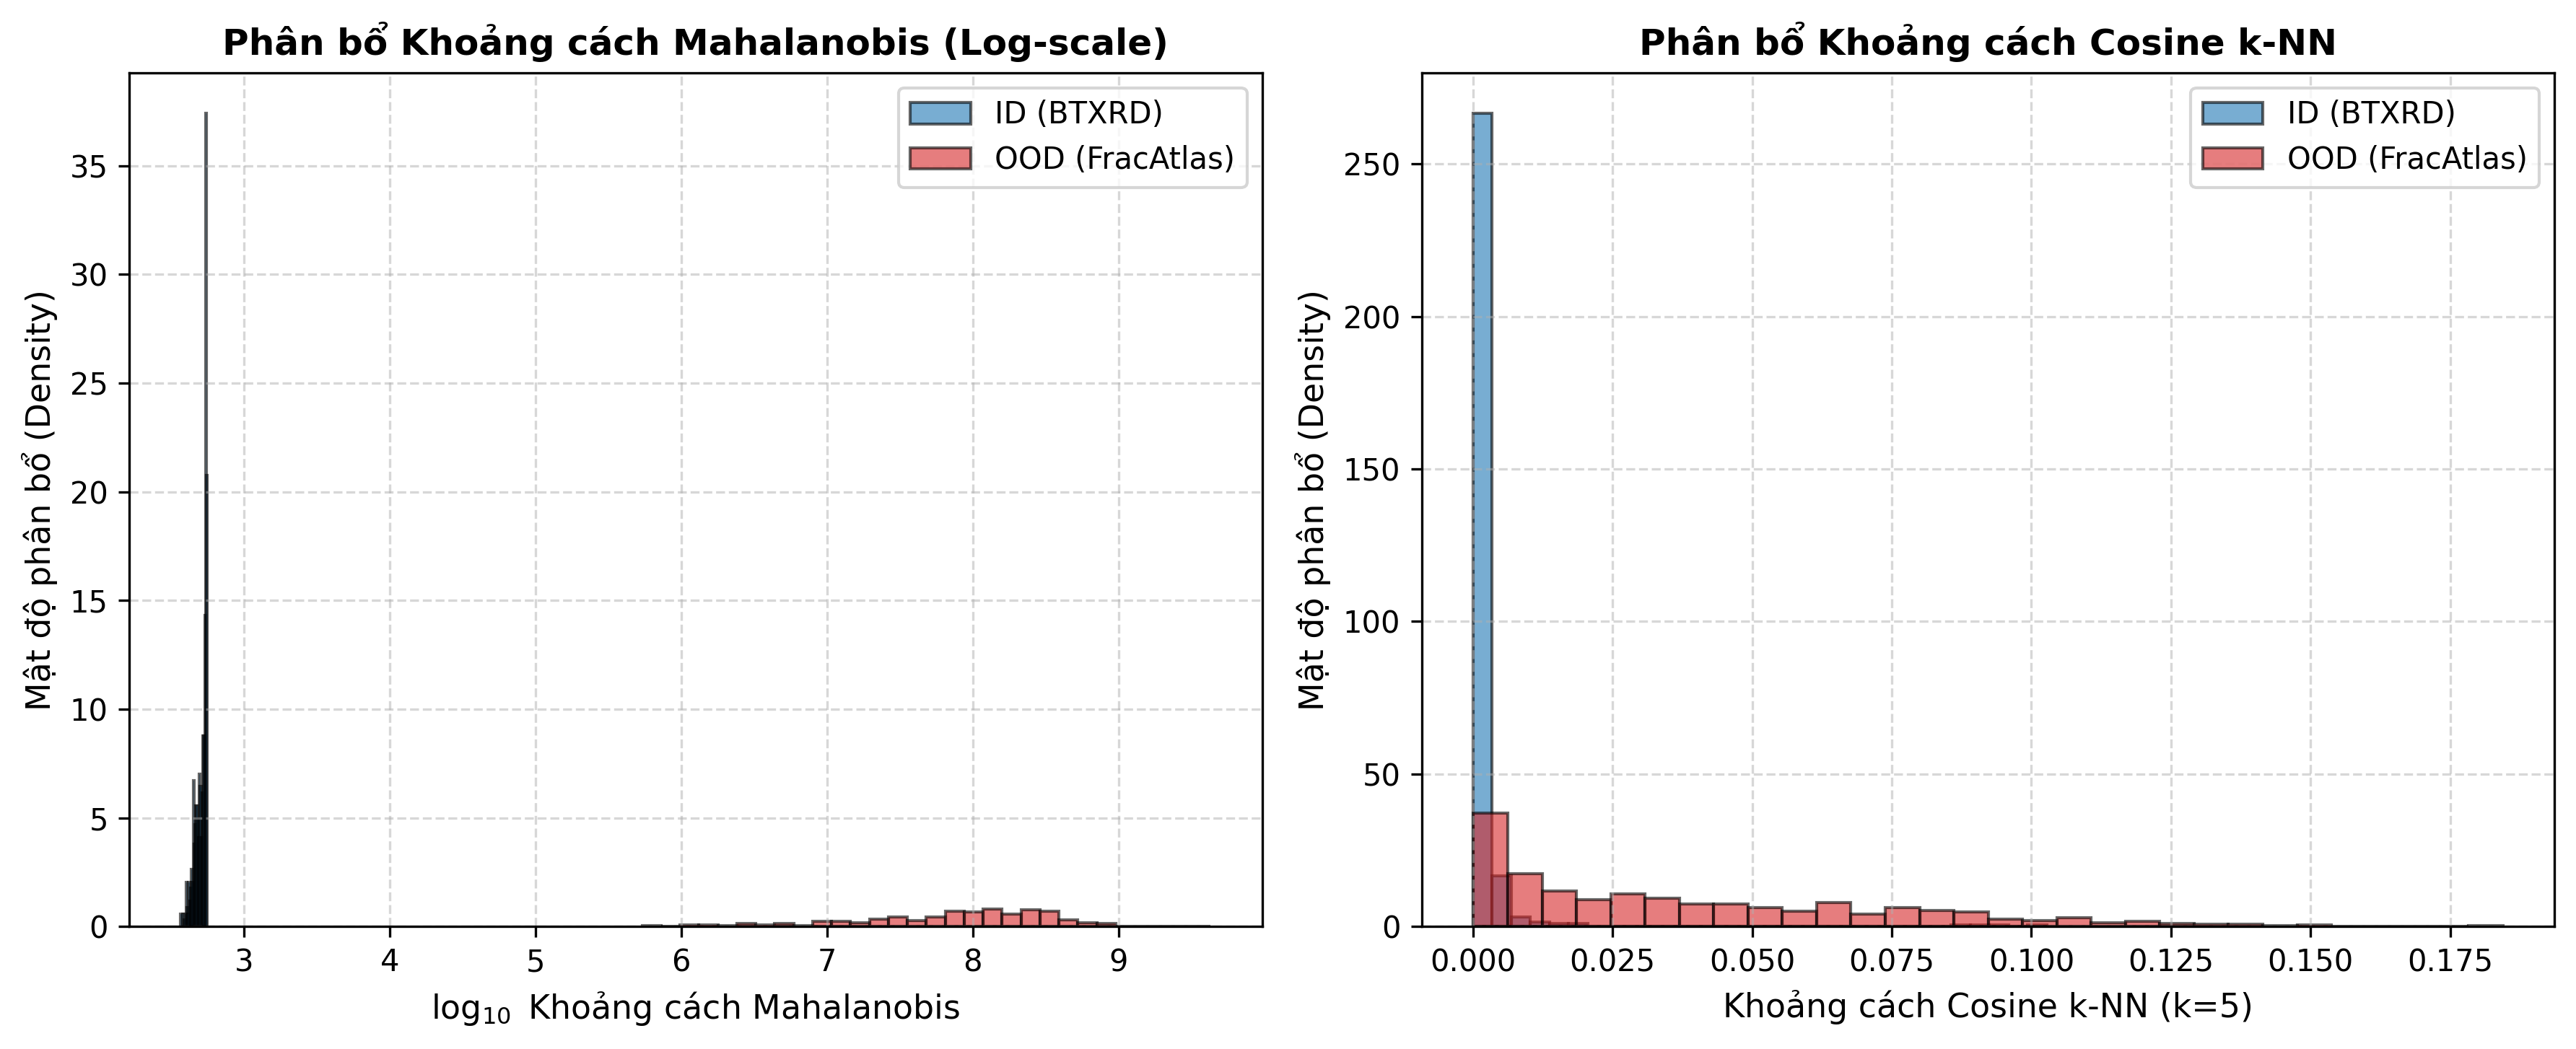
\includegraphics[width=0.95\textwidth]{images/ood_distribution.png}
% \caption{Biểu đồ phân bổ mật độ (Density Distribution) của khoảng cách Mahalanobis (trái) và khoảng cách Cosine k-NN (phải) đối với tập dữ liệu nội phân phối ID (BTXRD) và ngoài phân phối OOD (FracAtlas).}
% \label{fig:ood_distribution}
% \end{figure}


\subsection{Các thí nghiệm rời rạc}

Nhóm đã thực hiện các thí nghiệm loại bỏ thành phần để bóc tách đóng góp cụ thể của các mô-đun đề xuất trong kiến trúc XBone-Net.

Pipeline đề xuất được cố định theo Mục \ref{sec:final-pipeline} trước khi đọc kết quả ablation. Vì vậy, ablation không được dùng để tái định nghĩa mô hình đề xuất theo hướng hậu nghiệm. Nếu một cấu hình rút gọn đạt kết quả cao hơn, nghiên cứu báo cáo đầy đủ độ chênh lệch và xem đây là bằng chứng về điểm yếu hoặc sự đánh đổi của thành phần tương ứng (chẳng hạn hiệu năng ID, khả năng phát hiện OOD, chi phí tính toán hoặc độ ổn định giữa các hạt giống). Chỉ khi cấu hình đó được xác nhận lại bằng quy trình lựa chọn trên validation và đánh giá độc lập, nó mới có thể được xem là một phiên bản cải tiến trong nghiên cứu tiếp theo.

Ba bảng ablation dưới đây lưu lại các lần chạy thăm dò theo pipeline cũ nhằm
phục vụ truy vết. Các cấu hình này chưa kế thừa đầy đủ pipeline canonical, do đó
không được so sánh trực tiếp với Bảng \ref{tab:comparison_results} và không được
dùng để kết luận về đóng góp của từng thành phần. Bản báo cáo cuối cần thay các
giá trị này bằng kết quả chạy lại trên cùng split, ba hạt giống và cùng quy trình chọn
checkpoint.

\subsubsection{Đánh giá vai trò của các nguồn thông tin văn bản lâm sàng}
Mục đích thí nghiệm này là đánh giá tác động của việc tích hợp văn bản lâm sàng và cận lâm sàng đến kết quả chẩn đoán, đồng thời xác định xem có xảy ra hiện tượng rò rỉ nhãn hay không. Nhóm so sánh 4 kịch bản văn bản tại Bảng \ref{tab:ablation_text}.

\begin{table}[htbp]
\centering
\resizebox{\textwidth}{!}{
\caption{Kết quả thăm dò legacy về nguồn văn bản đầu vào; chưa dùng để kết luận}
\label{tab:ablation_text}
\begin{tabular}{|l|c|c|c|c|}
\hline
\textbf{Kịch bản văn bản} & \textbf{Văn bản sử dụng} & \textbf{F1-Macro} & \textbf{Accuracy} & \textbf{Macro AUROC} \\ \hline
Image only & Không sử dụng & 0,2052 & 0,6050 & 0,7857 \\ \hline
Image + clinical & Bệnh sử lâm sàng & 0,8583 & 0,9626 & 0,9869 \\ \hline
X-ray only & Mô tả kết quả X-quang & 1,0000 & 1,0000 & 1,0000 \\ \hline
Both texts & Lâm sàng + X-quang & 1,0000 & 1,0000 & 1,0000 \\ \hline
\end{tabular}
}
\end{table}

\textbf{Giới hạn diễn giải:} Kết quả hoàn hảo ở các hàng dùng báo cáo X-quang
phù hợp với nguy cơ rò rỉ nhãn vì văn bản có thể chứa tên bệnh. Tuy nhiên, các
giá trị legacy chưa đủ để định lượng riêng đóng góp của bệnh sử. Thí nghiệm
canonical cần so sánh image-only, clinical-only, image + clinical và image +
clinical bị xáo trộn trên cùng một checkpoint protocol.

\subsubsection{Đánh giá ảnh hưởng của chiến thuật tinh chỉnh backbone}
Mục đích thí nghiệm này là đánh giá hiệu năng khi đóng băng backbone so với
LoRA và tinh chỉnh toàn bộ trong cùng một quy trình huấn luyện. Hai hàng LoRA
trong bảng là cấu hình legacy, không phải thành phần của pipeline canonical.

\begin{table}[htbp]
\centering
\resizebox{\textwidth}{!}{
\caption{Kết quả thăm dò legacy về chiến thuật tinh chỉnh backbone; chưa dùng để kết luận}
\label{tab:ablation_finetuning}
\begin{tabular}{|c|c|c|c|c|}
\hline
\textbf{Chiến thuật} & \textbf{Pha 1} & \textbf{F1-Macro} & \textbf{Accuracy} & \textbf{Macro AUROC} \\ \hline
Đóng băng backbone & Không & 0,8095 & 0,9431 & 0,9907 \\ \hline
Tinh chỉnh LoRA & Có (Clinical) & 0,6140 & 0,8808 & 0,9665 \\ \hline
Tinh chỉnh toàn bộ & Có (Clinical) & 0,5951 & 0,8559 & 0,9632 \\ \hline
Tinh chỉnh LoRA (Gốc) & Có (Xray) & 0,6464 & 0,8754 & 0,9741 \\ \hline
\textbf{Tinh chỉnh LoRA (Cải tiến)} & \textbf{Có (Clinical)} & \textbf{0,8583} & \textbf{0,9626} & \textbf{0,9869} \\ \hline
\end{tabular}
}
\end{table}

\textbf{Giới hạn diễn giải:} Các hàng trong bảng đồng thời thay đổi chiến lược
tinh chỉnh, việc có chạy Pha 1 và nguồn văn bản, nên chênh lệch không thể quy
riêng cho LoRA, LoRA hay full fine-tuning. So sánh chính thức cần giữ cố định
nguồn văn bản, kiến trúc dung hợp, bộ phân loại và ngân sách huấn luyện.

\subsubsection{Đánh giá hiệu quả của đầu phân loại nguyên mẫu so với đầu phân loại tuyến tính}
Nhóm thí nghiệm này nhằm kiểm tra hiệu quả của đầu phân loại nguyên mẫu (Prototypical Head) so với đầu phân loại tuyến tính (Linear Head) truyền thống trong bài toán phân loại đa lớp u xương.

\begin{table}[htbp]
\centering
\resizebox{\textwidth}{!}{
\caption{Kết quả thăm dò legacy về bộ phân loại; chưa dùng để kết luận}
\label{tab:ablation_classifier}
\begin{tabular}{|l|c|c|c|c|}
\hline
\textbf{Backbone} & \textbf{Bộ phân loại} & \textbf{F1-Macro} & \textbf{Accuracy} & \textbf{Macro AUROC} \\ \hline
BiomedCLIP (Frozen) & Linear Head (B4) & 0,8105 & 0,9448 & 0,9940 \\ \hline
BiomedCLIP (Frozen) & Prototypical Head & 0,8095 & 0,9431 & 0,9907 \\ \hline
BiomedCLIP (LoRA) & Linear Head & 0,6261 & 0,8737 & 0,9693 \\ \hline
BiomedCLIP (LoRA) & Prototypical Head & 0,6464 & 0,8754 & 0,9741 \\ \hline
\end{tabular}
}
\end{table}

\textbf{Giới hạn diễn giải:} Bảng legacy sử dụng Prototypical Head của pipeline
cũ, trong khi mô hình canonical dùng empirical centroid. Kết luận về bộ phân
loại chỉ có thể được đưa ra sau khi so sánh linear head và empirical centroid
trên cùng encoder, cùng hạt giống và cùng hàm mất mát.

\subsection{Trực quan hóa bản đồ chú ý chéo và khả năng giải thích y khoa}
Để chứng minh khả năng giải thích lâm sàng (clinical explainability) và tính hợp lý về mặt y khoa của mô hình đề xuất XBone-Net, nhóm nghiên cứu tiến hành trích xuất bản đồ chú ý chéo (Cross-Attention Map) từ khối Transformer của mô-đun Cross-Attention Fusion cuối cùng trước đầu phân loại. Bản đồ này được thu nhận bằng cách tính toán trọng số tự chú ý (self-attention) của token đại diện lớp hình ảnh (CLS token) đối với các token vị trí hình ảnh (196 token patch), thể hiện mức độ tập trung của mô hình vào các vùng không gian trên ảnh chụp X-quang khi tổng hợp với thông tin bệnh sử lâm sàng.

Các kết quả trực quan hóa attention map chồng lên ảnh chụp X-quang gốc đối với một số nhóm bệnh lý điển hình từ tập kiểm thử được trình bày trong Hình \ref{fig:attention_visualizations}.

\begin{figure}[htbp]
\centering
\begin{tabular}{cc}
  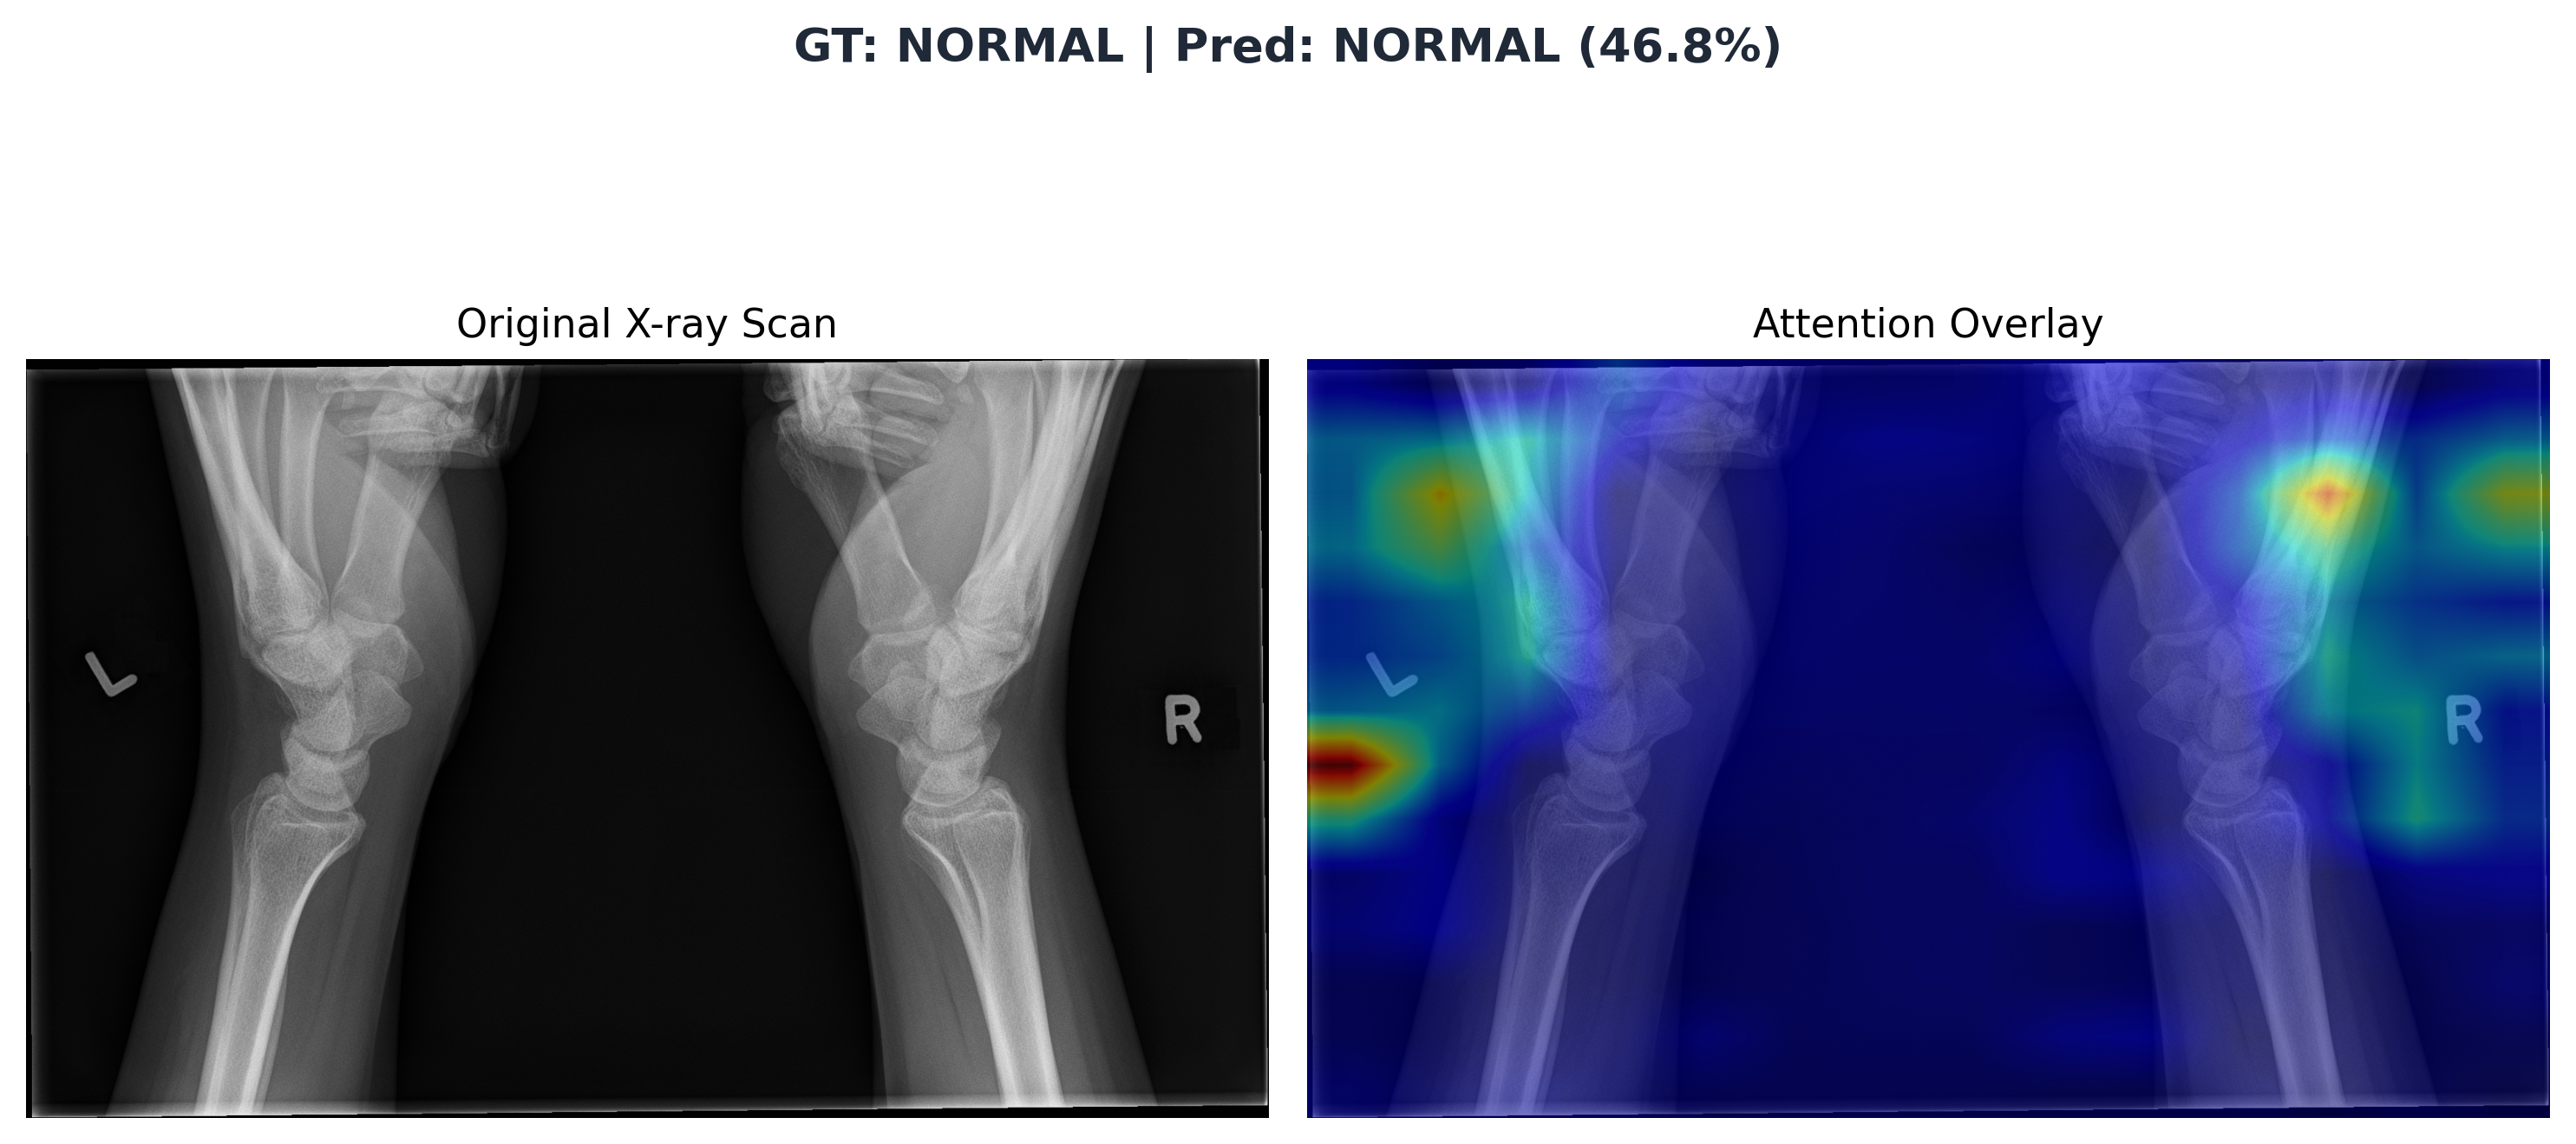
\includegraphics[width=0.48\textwidth]{images/attn_normal.png} &
  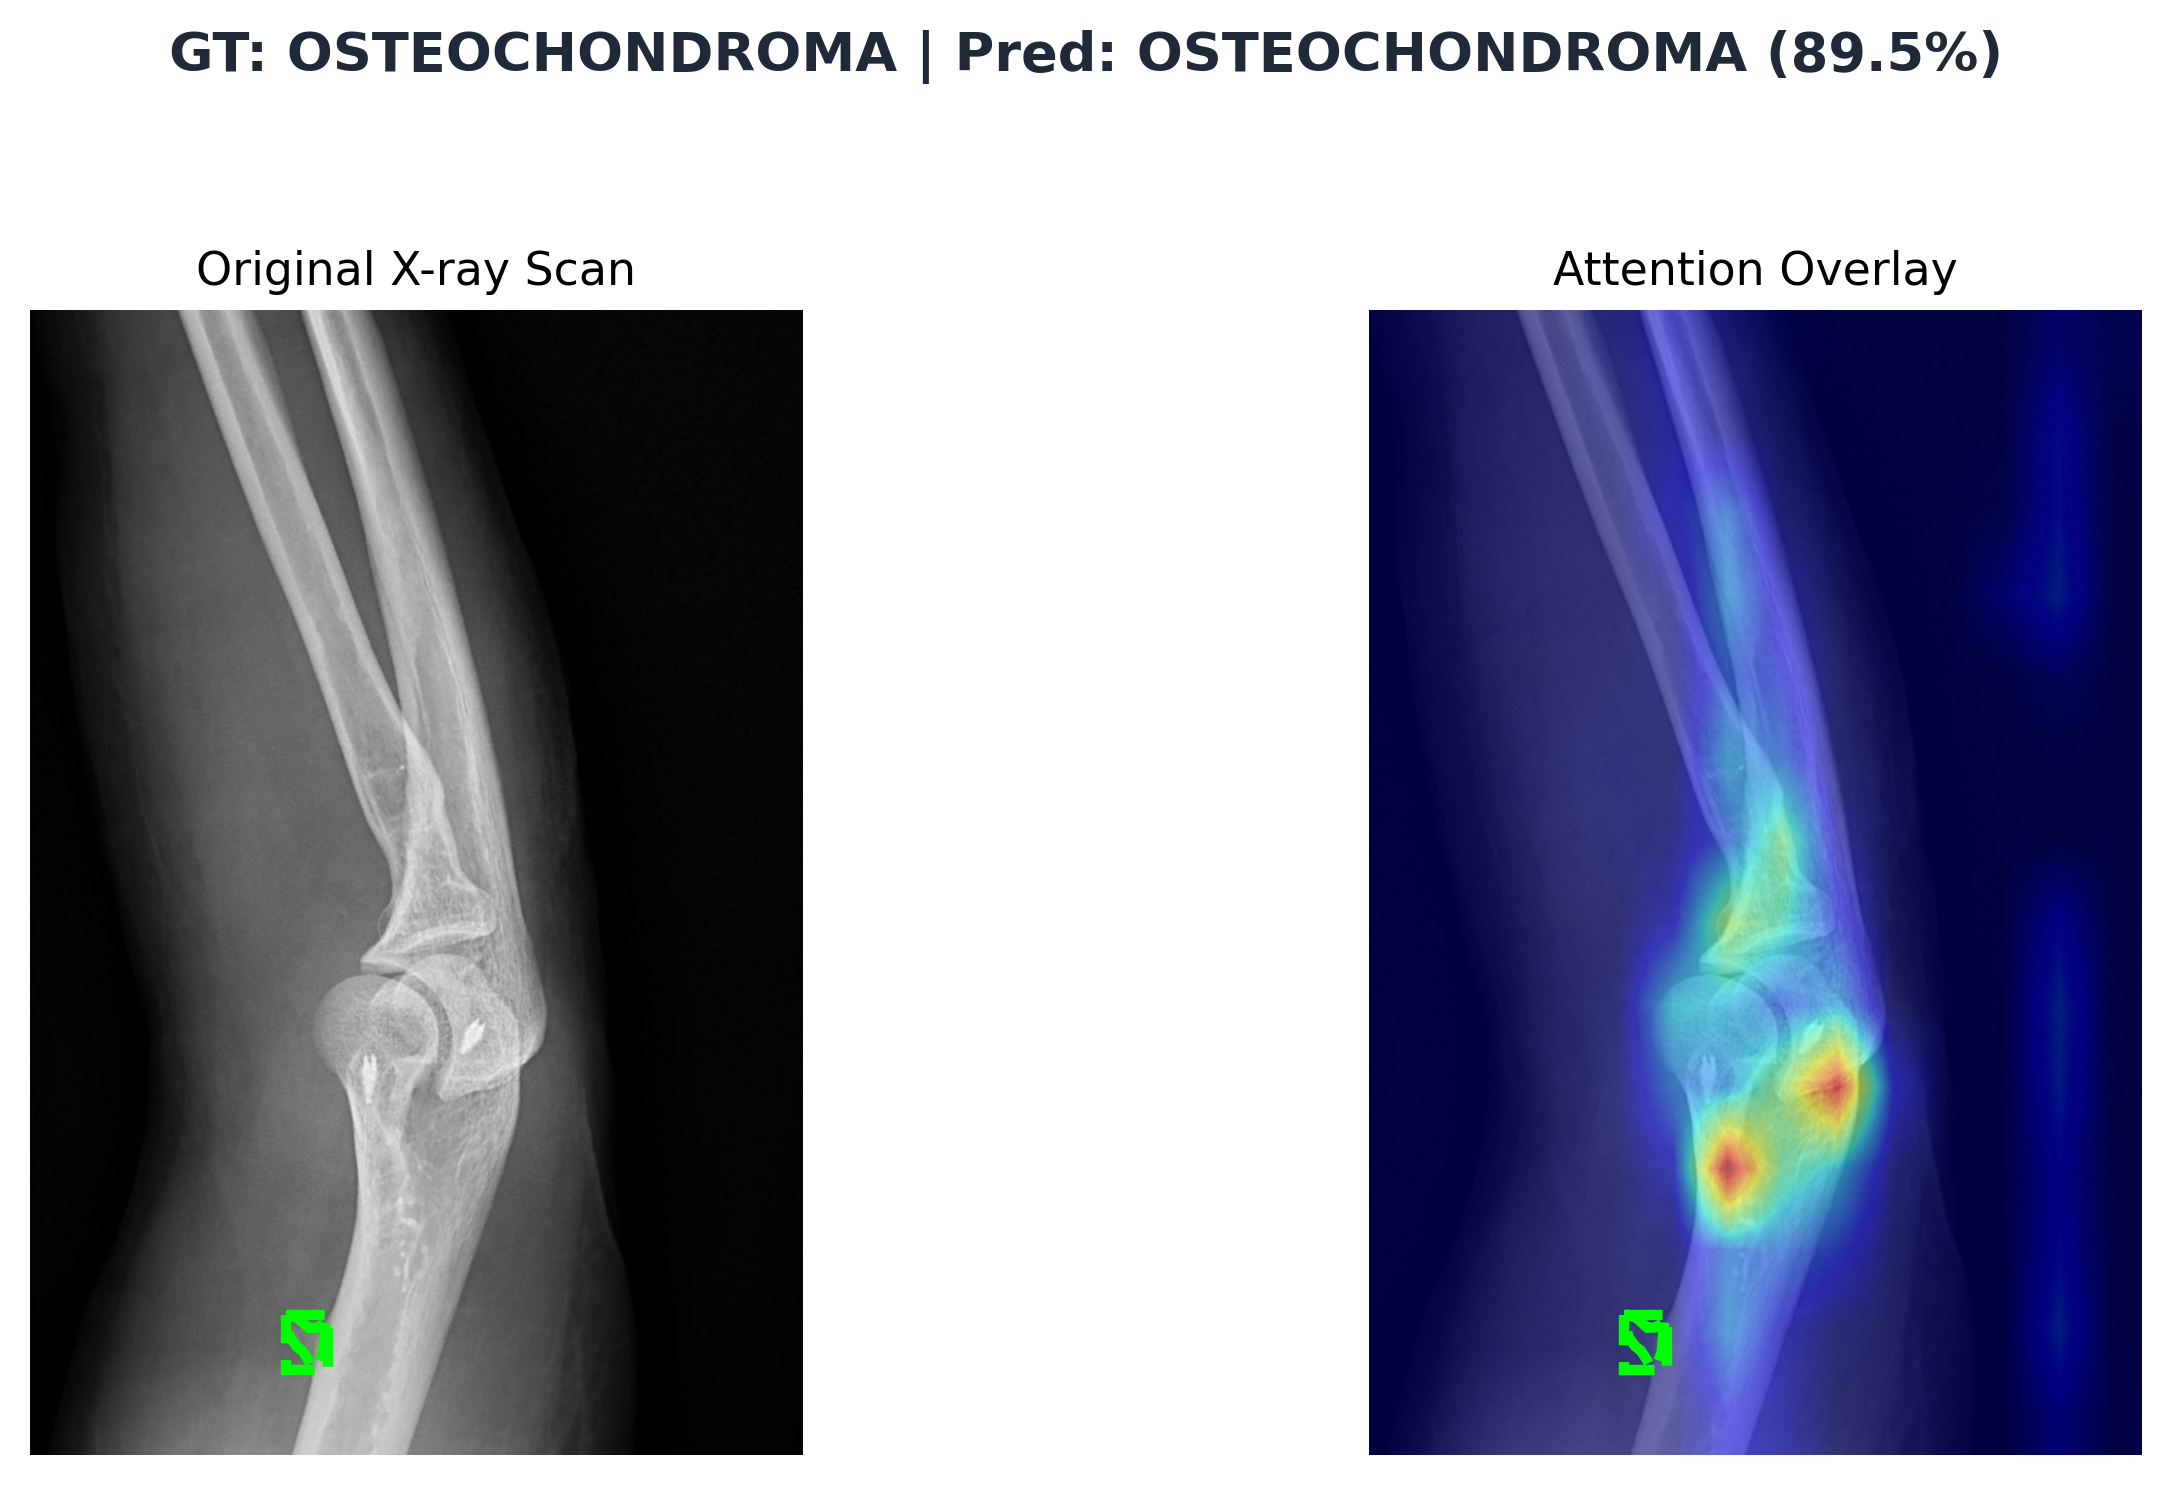
\includegraphics[width=0.48\textwidth]{images/attn_osteochondroma.png} \\
  (a) Mẫu bình thường (Normal) & (b) U xương sụn (Osteochondroma) \\
  \vspace{0.2cm} & \\
  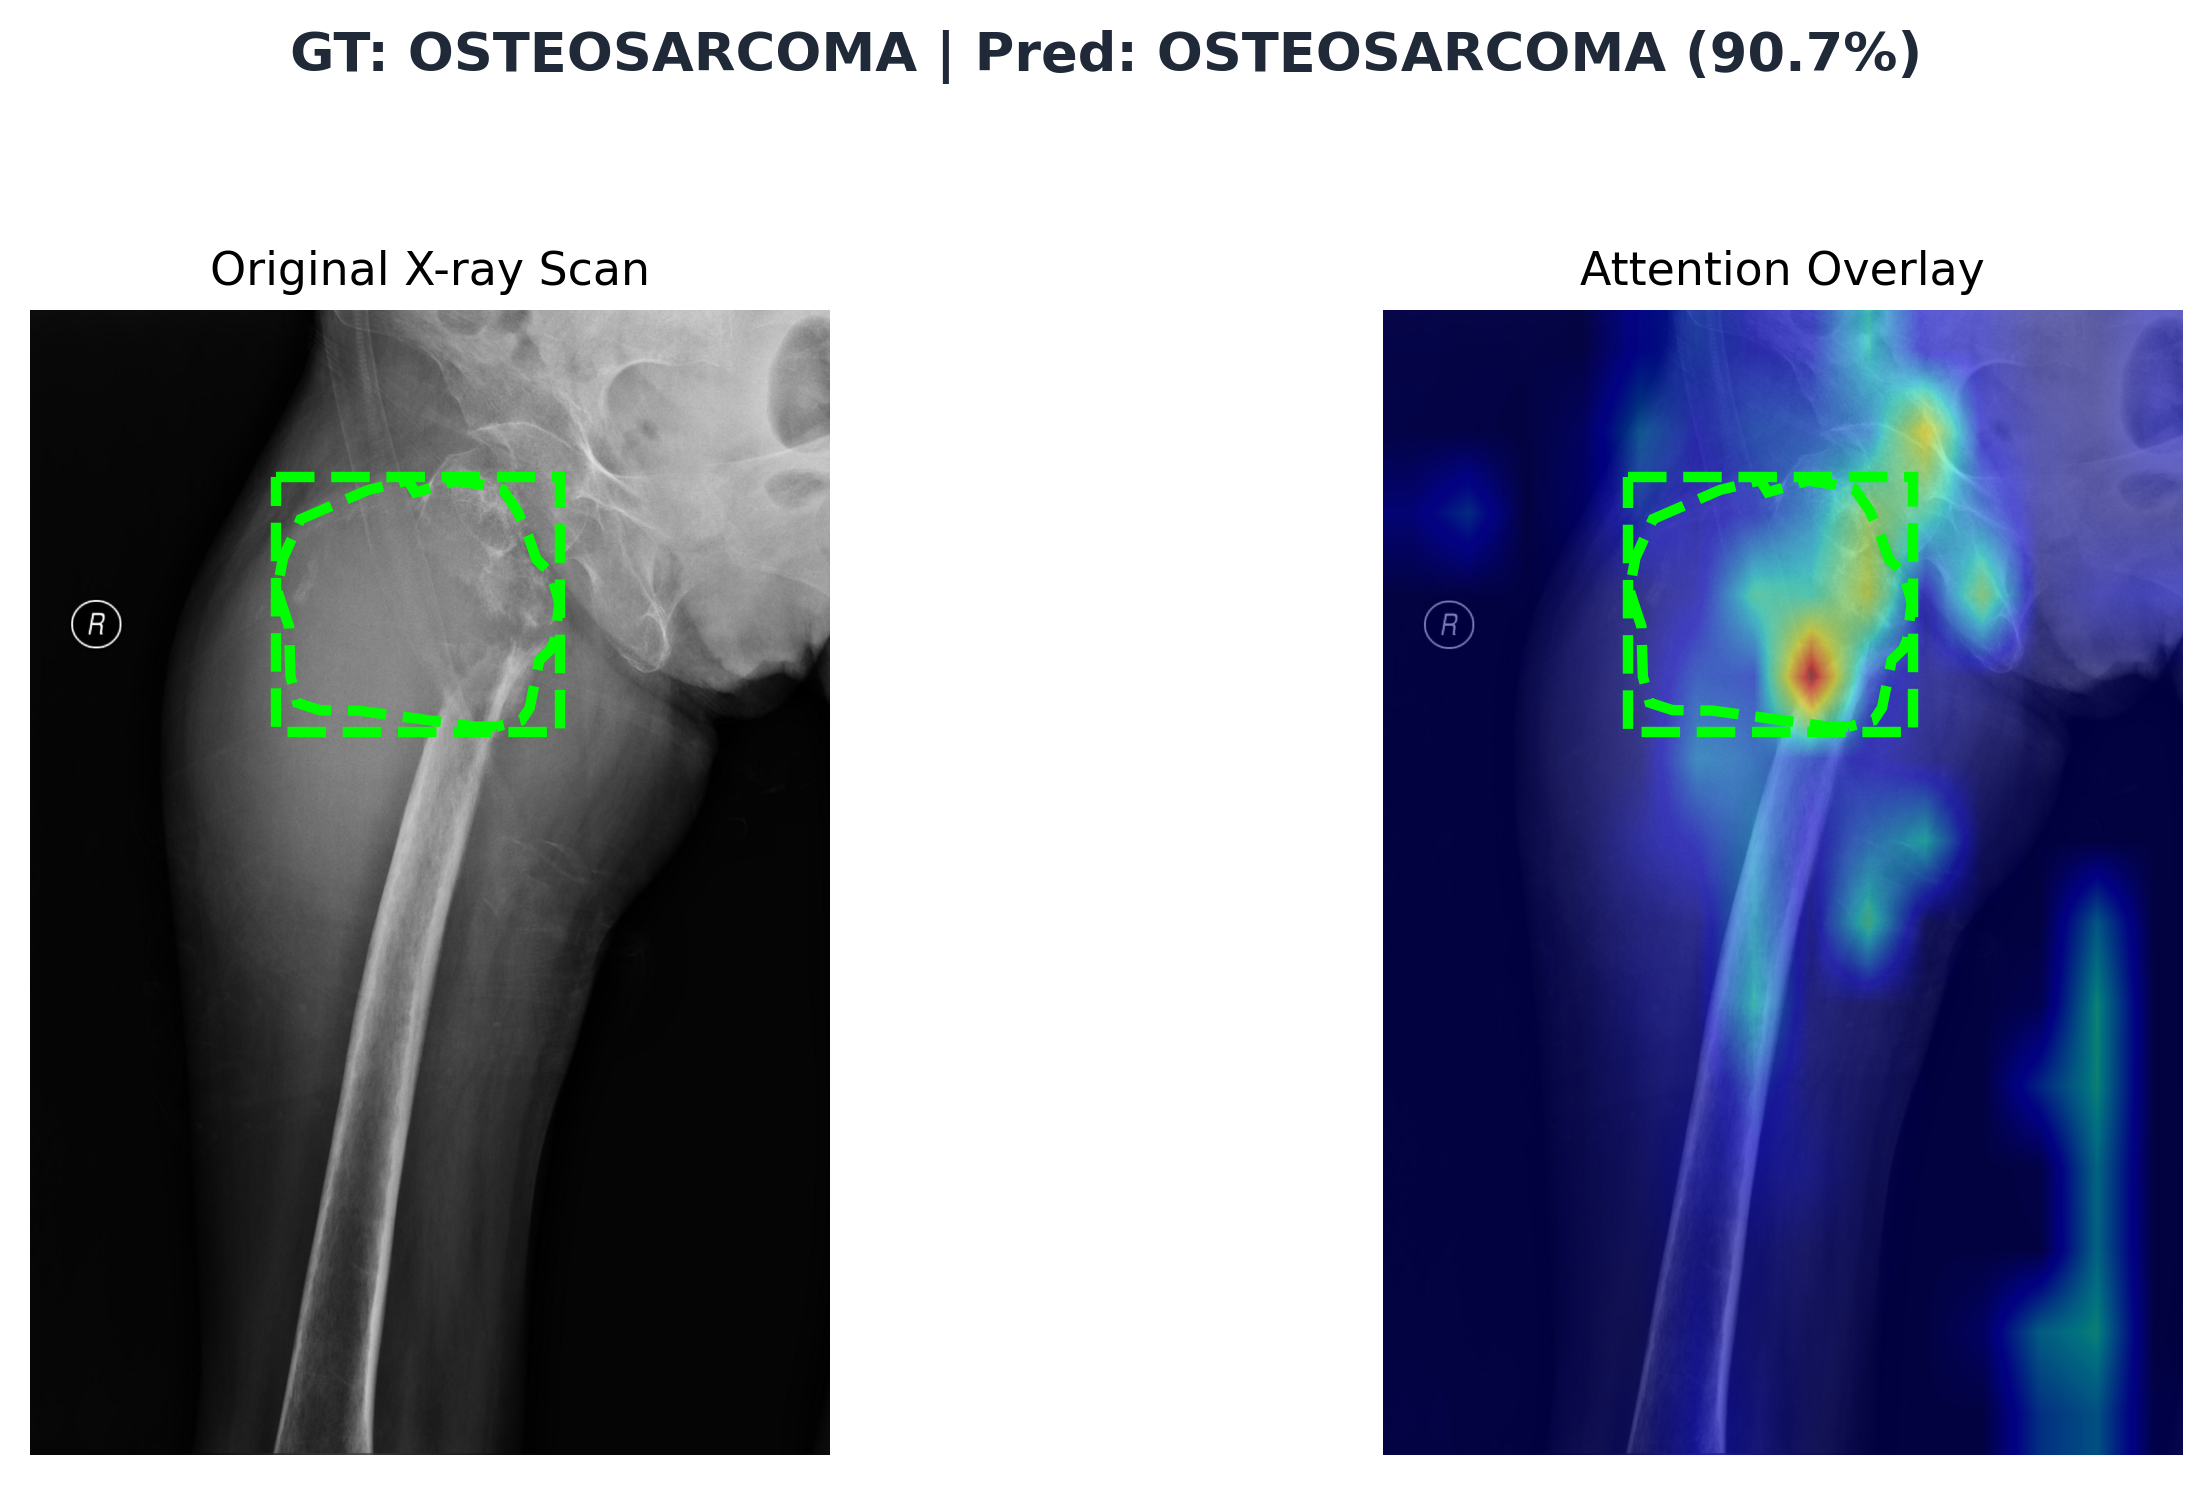
\includegraphics[width=0.48\textwidth]{images/attn_osteosarcoma.png} &
  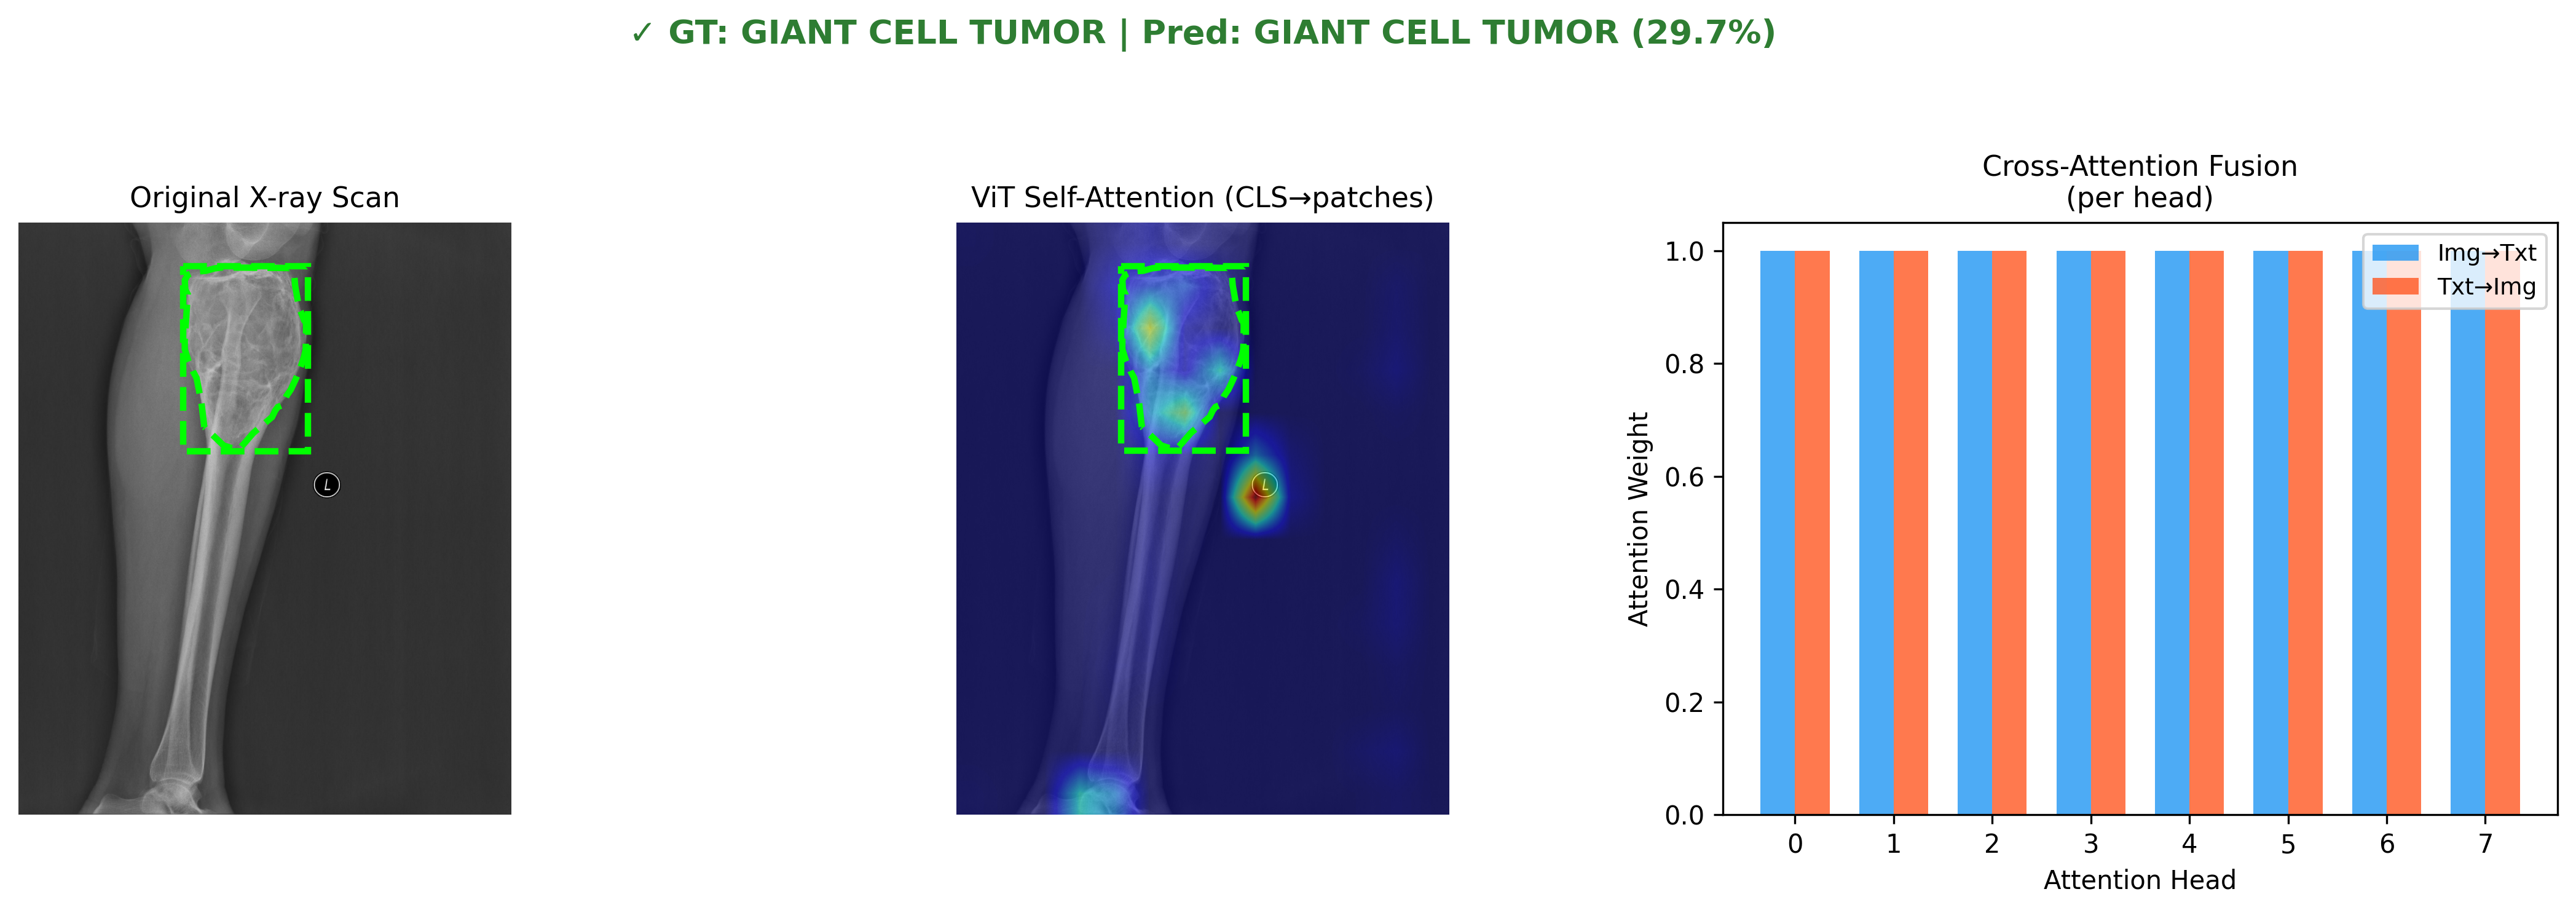
\includegraphics[width=0.48\textwidth]{images/attn_giant_cell_tumor.png} \\
  (c) Sarcoma xương (Osteosarcoma) & (d) U tế bào khổng lồ (Giant cell tumor) \\
\end{tabular}
\caption{Trực quan hóa bản đồ chú ý chéo (Cross-Attention Map) của mô hình đề xuất XBone-Net trên các nhóm bệnh lý điển hình (mỗi cặp gồm ảnh chụp X-quang gốc bên trái đã vẽ đường nét đứt màu xanh lá thể hiện phân vùng tổn thương thực tế - Ground Truth và ảnh chồng bản đồ chú ý chéo ở bên phải).}
\label{fig:attention_visualizations}
\end{figure}

\textbf{Phân tích định tính y khoa và kết quả định lượng:}
\begin{itemize}
    \item \textbf{Trường hợp Bình thường (Hình \ref{fig:attention_visualizations}a):} Đối với ca chẩn đoán bình thường không có khối u xương (Normal), mô hình đề xuất dự đoán chính xác nhãn NORMAL với độ tự tin đạt \textbf{46,8\%}. Bản đồ chú ý chéo cho thấy trọng số chú ý không tập trung vào bất kỳ vùng khu trú bất thường nào, mà phân bổ rộng rãi, đồng đều và mờ nhạt trên toàn bộ vùng giải phẫu của đầu dưới xương đùi và khớp gối. Điều này phản ánh sự tương khớp hoàn toàn với thực tế lâm sàng khi không có bất kỳ tổn thương hay cấu trúc khối u cục bộ nào cần phải khoanh vùng.
    \item \textbf{Trường hợp U xương sụn (Hình \ref{fig:attention_visualizations}b):} Đối với bệnh lý u xương sụn (Osteochondroma), mô hình dự đoán chính xác lớp OSTEOCHONDROMA với độ tự tin rất cao đạt \textbf{89,5\%}. Bản đồ chú ý của mô hình tập trung cực kỳ chính xác vào phần chồi xương nhô ra từ bề mặt hành xương đùi (exostosis) - đây chính là vùng tổn thương giải phẫu bệnh lý đặc trưng nhất của loại u này, hoàn toàn trùng khớp với phân vùng tổn thương thực tế (Ground Truth) được khoanh bằng đường nét đứt màu xanh lá.
    \item \textbf{Trường hợp Sarcoma xương (Hình \ref{fig:attention_visualizations}c):} Sarcoma xương (Osteosarcoma) là một khối u ác tính có tính chất hủy xương và xâm lấn mạnh. Mô hình XBone-Net đã nhận diện chính xác bệnh lý này với độ tự tin rất cao đạt \textbf{90,7\%}. Bản đồ trực quan hóa cho thấy mô hình tập trung mạnh mẽ và chính xác vào vùng hủy xương ở đầu dưới xương đùi kèm theo phản ứng màng xương dạng thớ (Sunburst/Codman triangle), chứng minh mô hình có khả năng định vị rất tốt các dấu hiệu nguy kịch của bệnh lý ác tính này.
    \item \textbf{Trường hợp U tế bào khổng lồ (Hình \ref{fig:attention_visualizations}d):} Ở trường hợp u tế bào khổng lồ (Giant cell tumor), mô hình chẩn đoán chính xác lớp GIANT CELL TUMOR với độ tự tin đạt \textbf{27,7\%}. Mặc dù đây là lớp bệnh lý hiếm gặp dẫn đến độ tự tin thấp hơn, bản đồ chú ý chéo vẫn tập trung rất rõ rệt vào vùng đầu xương (epiphysis) giáp khớp gối - vị trí tổn thương đặc hữu dạng "bong bóng xà phòng" (soap bubble appearance) của loại u này, trùng khớp với vùng chú thích Ground Truth.
\end{itemize}

Các kết quả định tính trên chứng minh rằng mô hình XBone-Net không chỉ đưa ra các dự đoán phân loại dựa trên các tương quan thống kê thuần túy, mà đã thực sự học được cách liên kết chặt chẽ thông tin gợi ý từ bệnh sử lâm sàng để định vị đúng các vùng tổn thương giải phẫu bệnh lý thực tế trên ảnh X-quang, mang lại giá trị giải thích cao và củng cố niềm tin cho các y bác sĩ trong quá trình hỗ trợ chẩn đoán.
\fi
\fi
